%-----------------------------------------------------------------------------%
\chapter{Performance Evaluation}
%-----------------------------------------------------------------------------%
%---------------------------------------------------------------

\section{Simulation Setup}




The proposed scheme was tested in a real network environment using an NS3 network simulator with TSCH model that is developed by European Institute of Innovation \& Technology (EIT-ICT) \cite{tschweb, 7820597}. A WSNs consisting of 20 sensor nodes and one sink node with a star topology and mesh topology (4 out of 20 nodes are cluster head in a mesh topology), as shown in Fig.\ref{fig:kodok} and Fig. \ref{fig:kodok} were considered. The buffer capacity of each node was set to 30 KB. Moreover, the sampling time was 1 $s$.  The IEEE 802.15.4e  TSCH MAC protocol with the two-ray ground radio propagation model is used. Each sensor node transmitted the packet to the sink node with the transmission rate starting from 1 KBps. Every simulation parameter is provided in Table \ref{my-label3}.

In this thesis, each node can only transmit in one of eighteen levels of data rate. Those data rate are $500, 1500, 2000, 2500, ..., 8000$ Kbytes/s. Therefore every second, calculated transmission rate corresponds to the closest available data rate. 

\begin{table}
	\centering
	\caption{Simulation Parameters}
	\label{my-label3}
	\begin{tabular}{|l|r|}
		\hline
		\multicolumn{1}{|c|}{Parameter} & \multicolumn{1}{c|}{Value} \\ \hline
		MAC layer                       & IEEE 802.15.4e  TSCH       \\ \hline
		PHY layer                       & IEEE 802.15.4 PHY          \\ \hline
		Radio propagation               & Two-way gorund             \\ \hline
		Intial data rate                & 1 KBps                     \\ \hline
		Packet size                     & 1024 bit                   \\ \hline
		Number of node                  & 20                         \\ \hline
		Buffer capacity                 & 30 KB                      \\ \hline
		Sampling time                   & 1 s                        \\ \hline
		Topology                        & Star, Mesh                 \\ \hline
		Duty cycle                      & 0.45 and 0.1               \\ \hline
		Simulation Time                 & 400s                       \\ \hline
		Number of agent                 & 10                         \\ \hline
		$MaxIteration$                  & 5                          \\ \hline
	\end{tabular}
\end{table}

\section {Simulation Results}

In this scheme, due to the coexistence solution in C-LV model, congestion is always guaranteed. However, the end-to-end delay needs improvement. DA is applied in the C-LV model to minimize the end-to-end delay of each node while transmitting data to the sink node while maintaining fairness and stability. Therefore in this thesis, throughput and stability are considered as the primary metric of this scheme.

As explained before, DA minimizes the end-to-end delay by finding the highest transmission rate possible without any possibility of congestion while maintaining the stability. DA needs only the number of sensor nodes that actively send packets to the sink node. Therefore, if there is a change in the number of active sensor nodes, DA needs to be applied to find closest to the optimal solution of each particular number of sensor nodes. As shown in Fig.~\ref{fig:of}, it takes less than five iterations for the DA find the solution; thus, it does not take any significant time to find the solution.

\begin{figure}
	\centering
	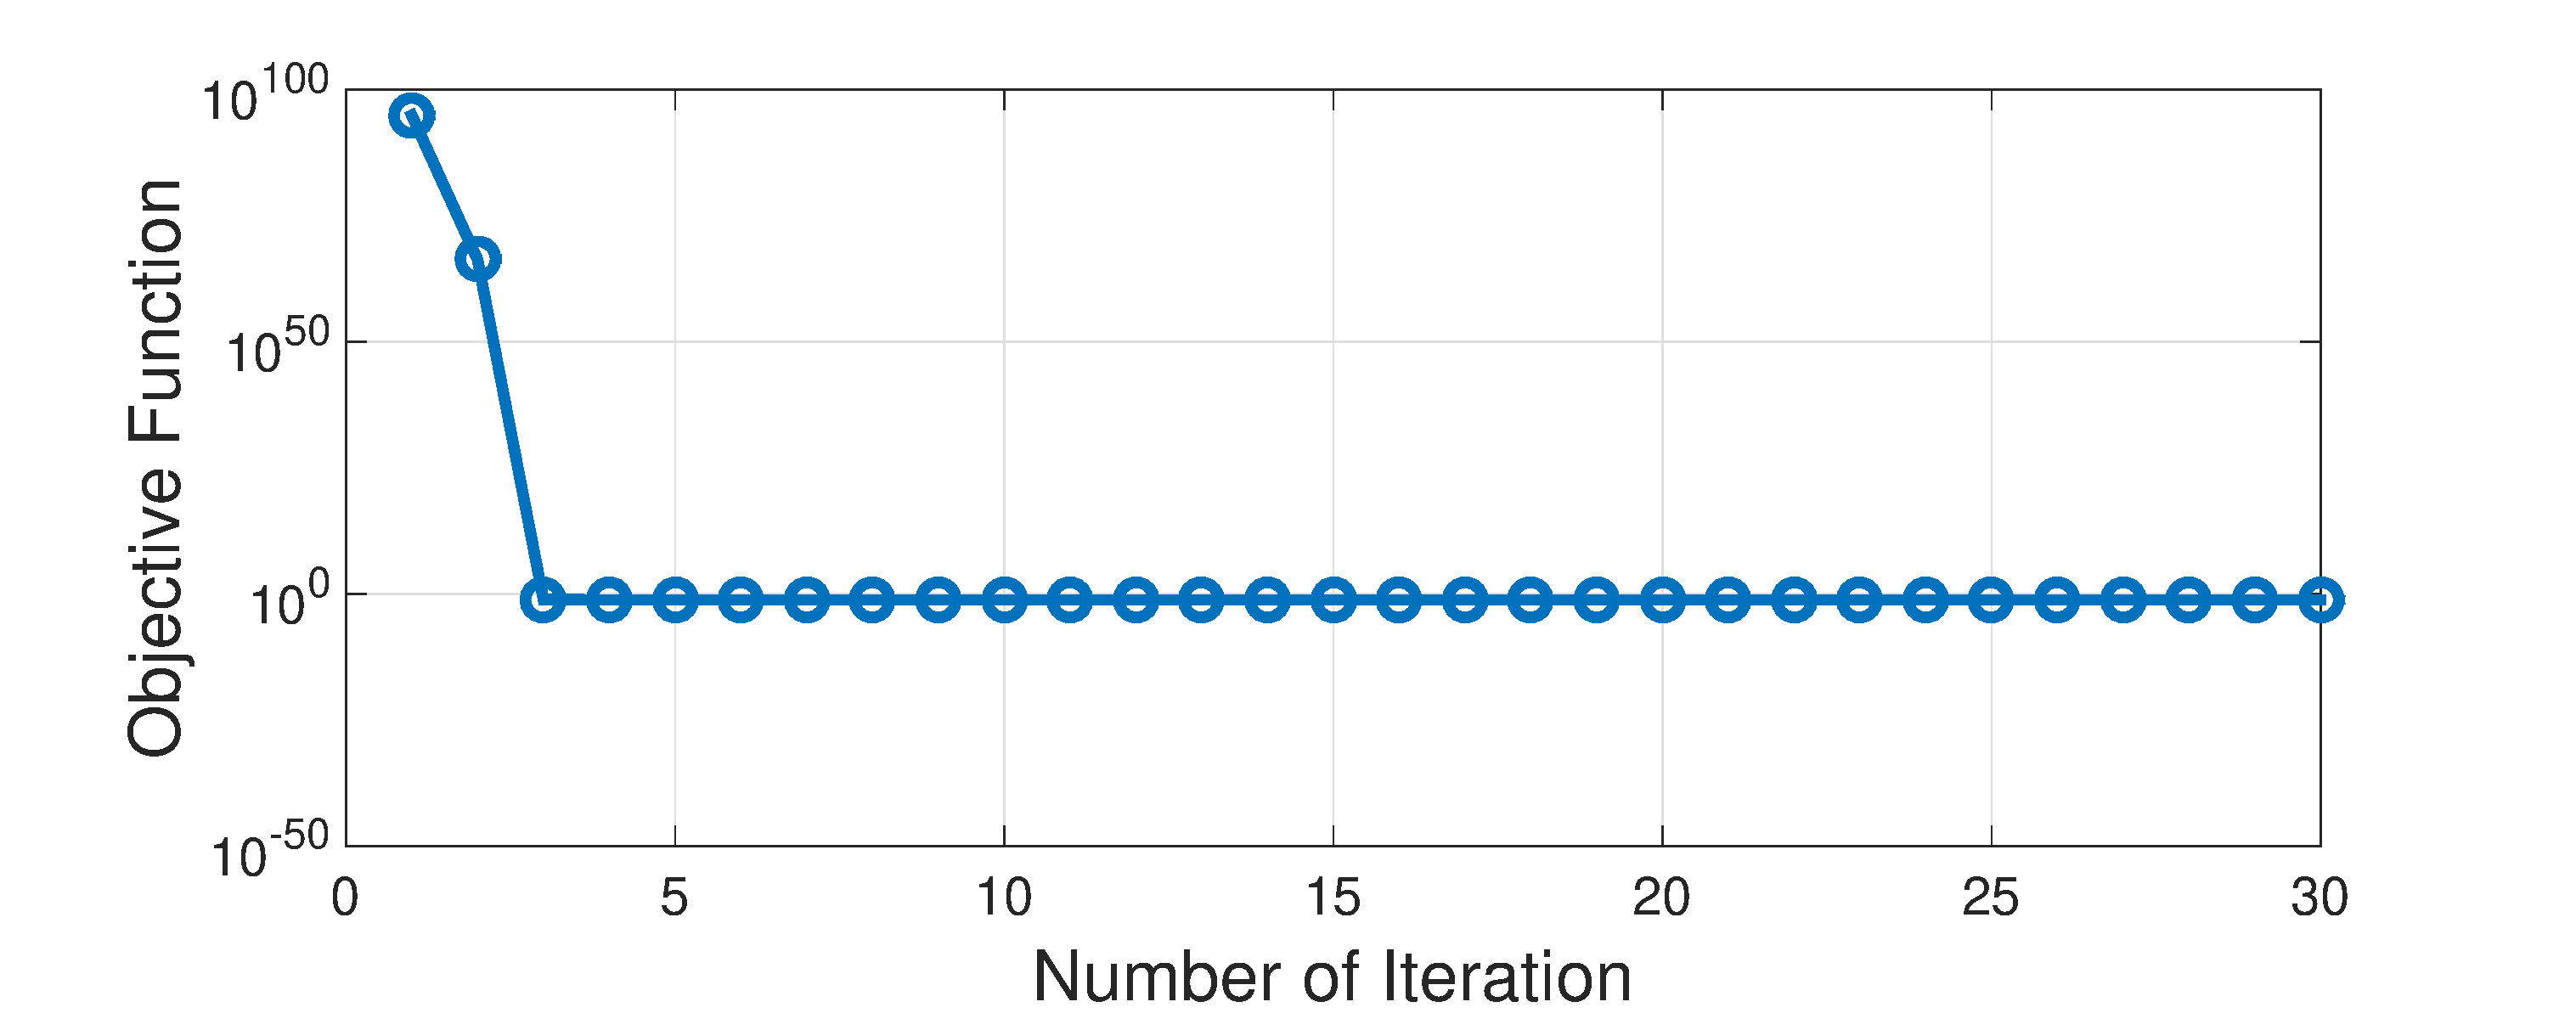
\includegraphics[width=1\linewidth]{pics/of}
	\caption{Objective Function over Number of Iteration}
	\label{fig:of}
\end{figure}

A particular scenario was considered to evaluate the performance of the proposed algorithms. Two scenarios are investigated. The first scenario was conducted for star topology. At first, there only five active sensor nodes (sensor node 1-5). Every 100 seconds, another five sensor nodes are activated. This scheme continues until all 20 sensor nodes are activated. Through this scenario, the adaptiveness of the hybrid scheme could be assessed. In addition, in this scenario, the proposed scheme is compared with another congestion control Additive increase/multiplicative decrease (AIMD). For the second scenario, evaluation in mesh topology was conducted. At first, there only four active sensor nodes (sensor node 1-4) which are under cluster head 1. Similar to the first scenario, every 100 seconds, four sensor nodes from another cluster head are activated. This scheme continues until all 16 sensor nodes, and 4 cluster heads are activated. This scenario shows that proposed method can be used for every topology with predefined routing path. In these two scenarios, all sensor nodes have the same priority. However, a scenario with different priority was also conducted.

\subsection{Simulation Result With Star Topology}



The results are shown in Fig. \ref{fig:lotka} and Fig. \ref{fig:lotkatru} demonstrate that the scheme is adaptive and nearly optimal. Where Fig. \ref{fig:lotka} shows the calculated transmission rate from particular node and Fig. \ref{fig:lotkatru} shows throughput of particular node measured from the sink node. Even with a harsh industrial environment, recorded throughput showed a similar result with the calculated transmission rate with delay and small noises. As shown in Fig. \ref{fig:lotkatru}, noise gets stronger as the number of nodes increased due to interference. However, nearly optimal and stable result is shown.
The transmission rate is changed rapidly based on the number of sensor nodes. The Proof that this scheme is nearly optimal is shown in Fig. \ref{fig:lotka1}. In that time, there only 5 active sensor nodes and the buffer capacity is 30 KB. All five sensor nodes transmit nearly 6 KBps without any congestion occurring in the network. Fig. \ref{fig:lotka2} shows how fast the scheme adapts when the number of active nodes is increased to 10. When a steady state is achieved, all ten sensor nodes transmit at a rate of nearly 3 KBps. It should be noted that DA works every time there is a change in the number of nodes; thus, this scheme adapts to changing conditions quickly and optimally. To strengthen the proof that DA enhance the C-LV scheme for congestion control, Fig. \ref{fig:comp1} shows the comparative evaluation between 
C-LV scheme for congestion control with DA (Adaptive) and without DA (Non-Adaptive). When the number of nodes is increased, the calculated transmission rate of non-adaptive C-LV oscillates with high frequency. Moreover, after $300$ \textit{s}, the calculate transmission rate goes extinct because the instability.
%\begin{figure}
%	\centering
%	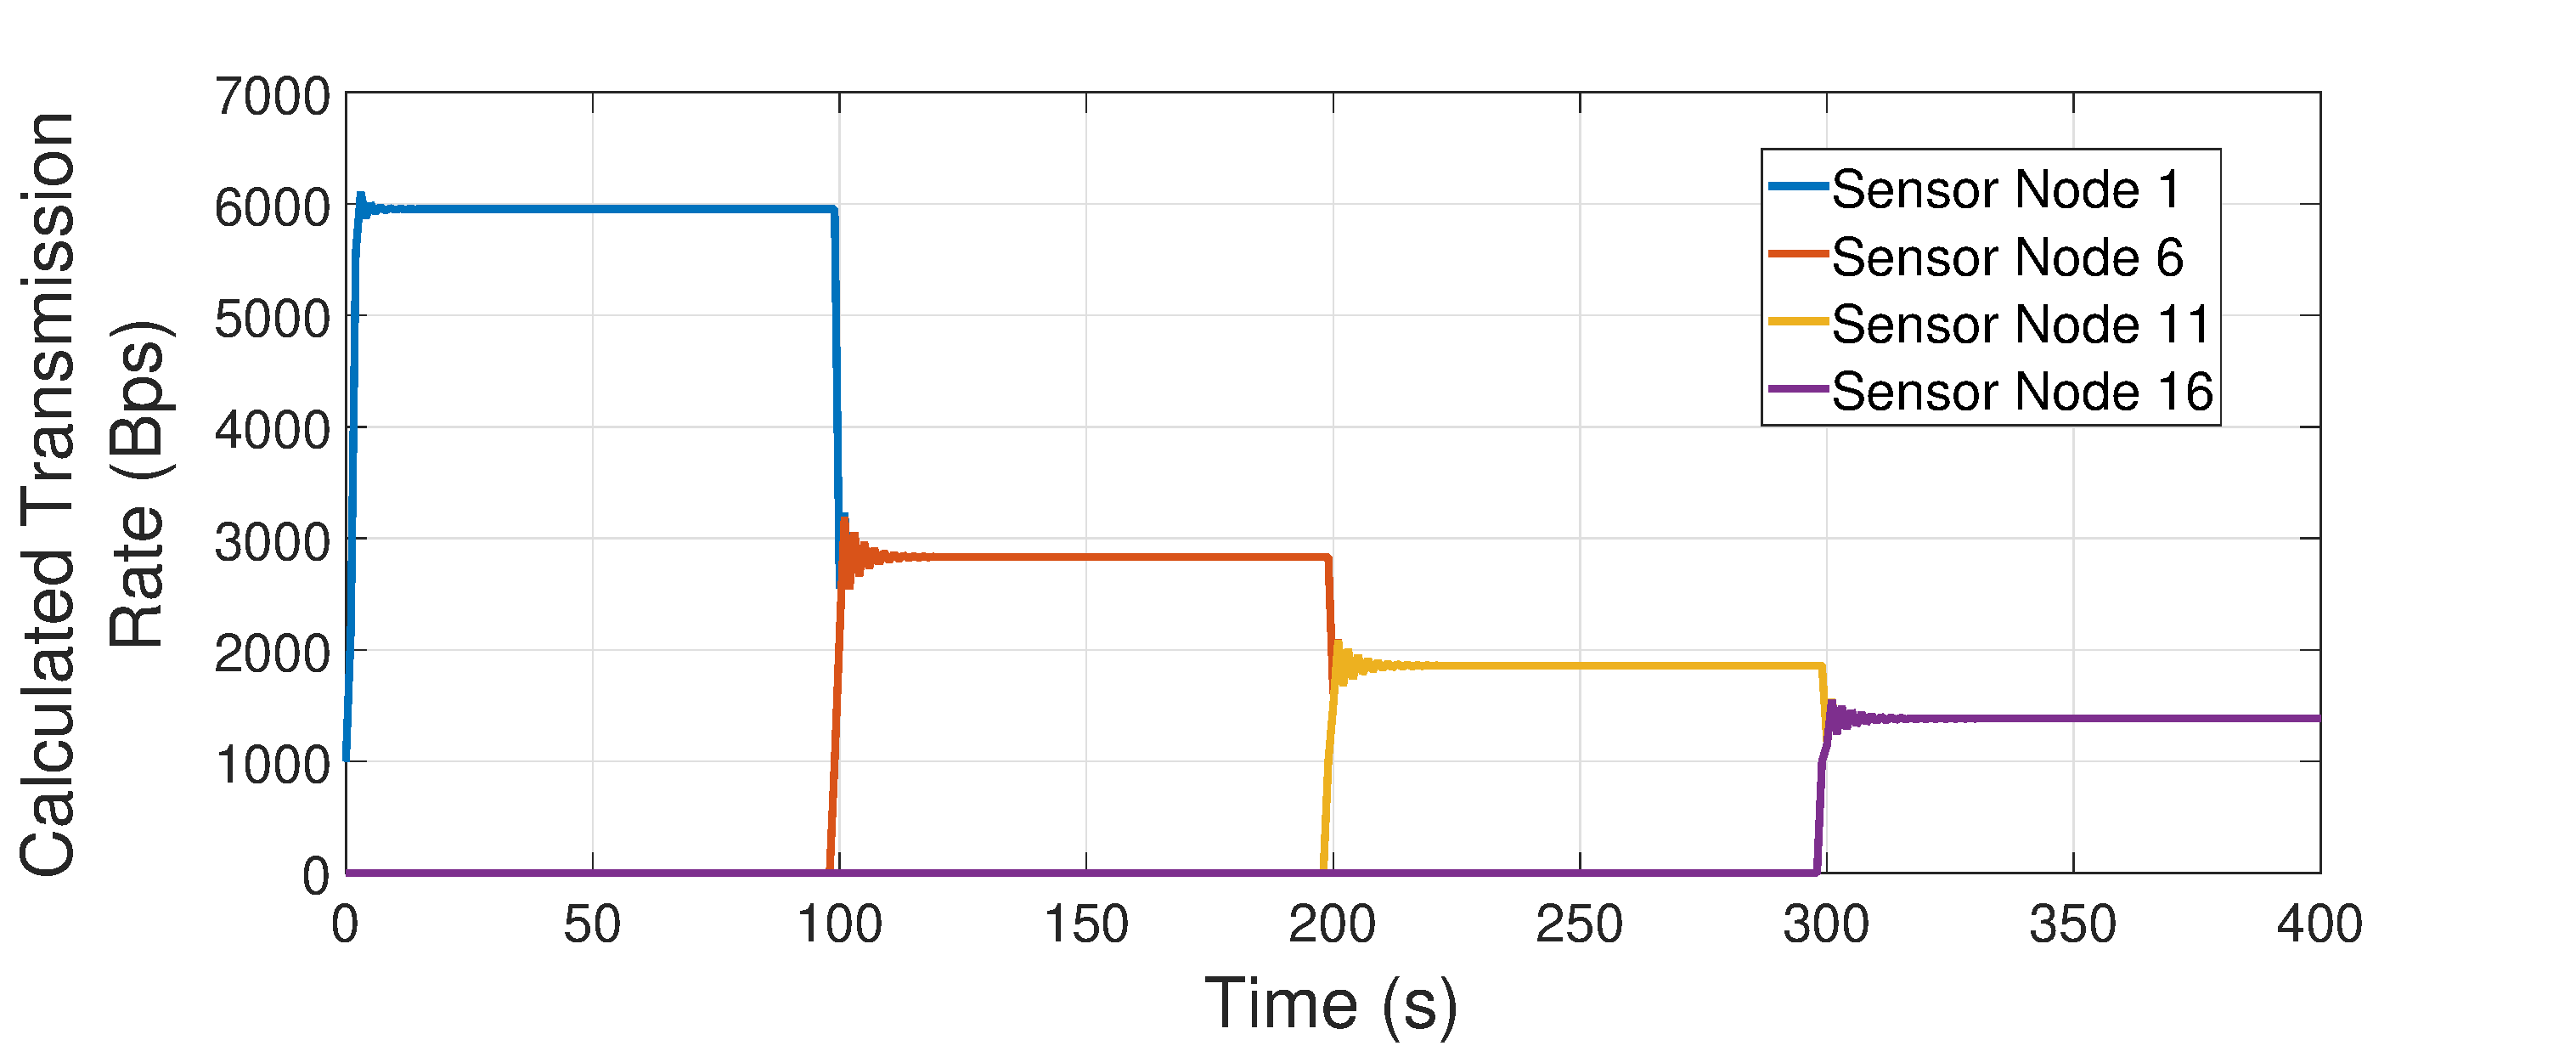
\includegraphics[width=1\linewidth]{pics/Lotka}
%	\caption{Transmission Rate with star topology}
%	\label{fig:lotka}
%\end{figure}
%
%\begin{figure}
%	\centering
%	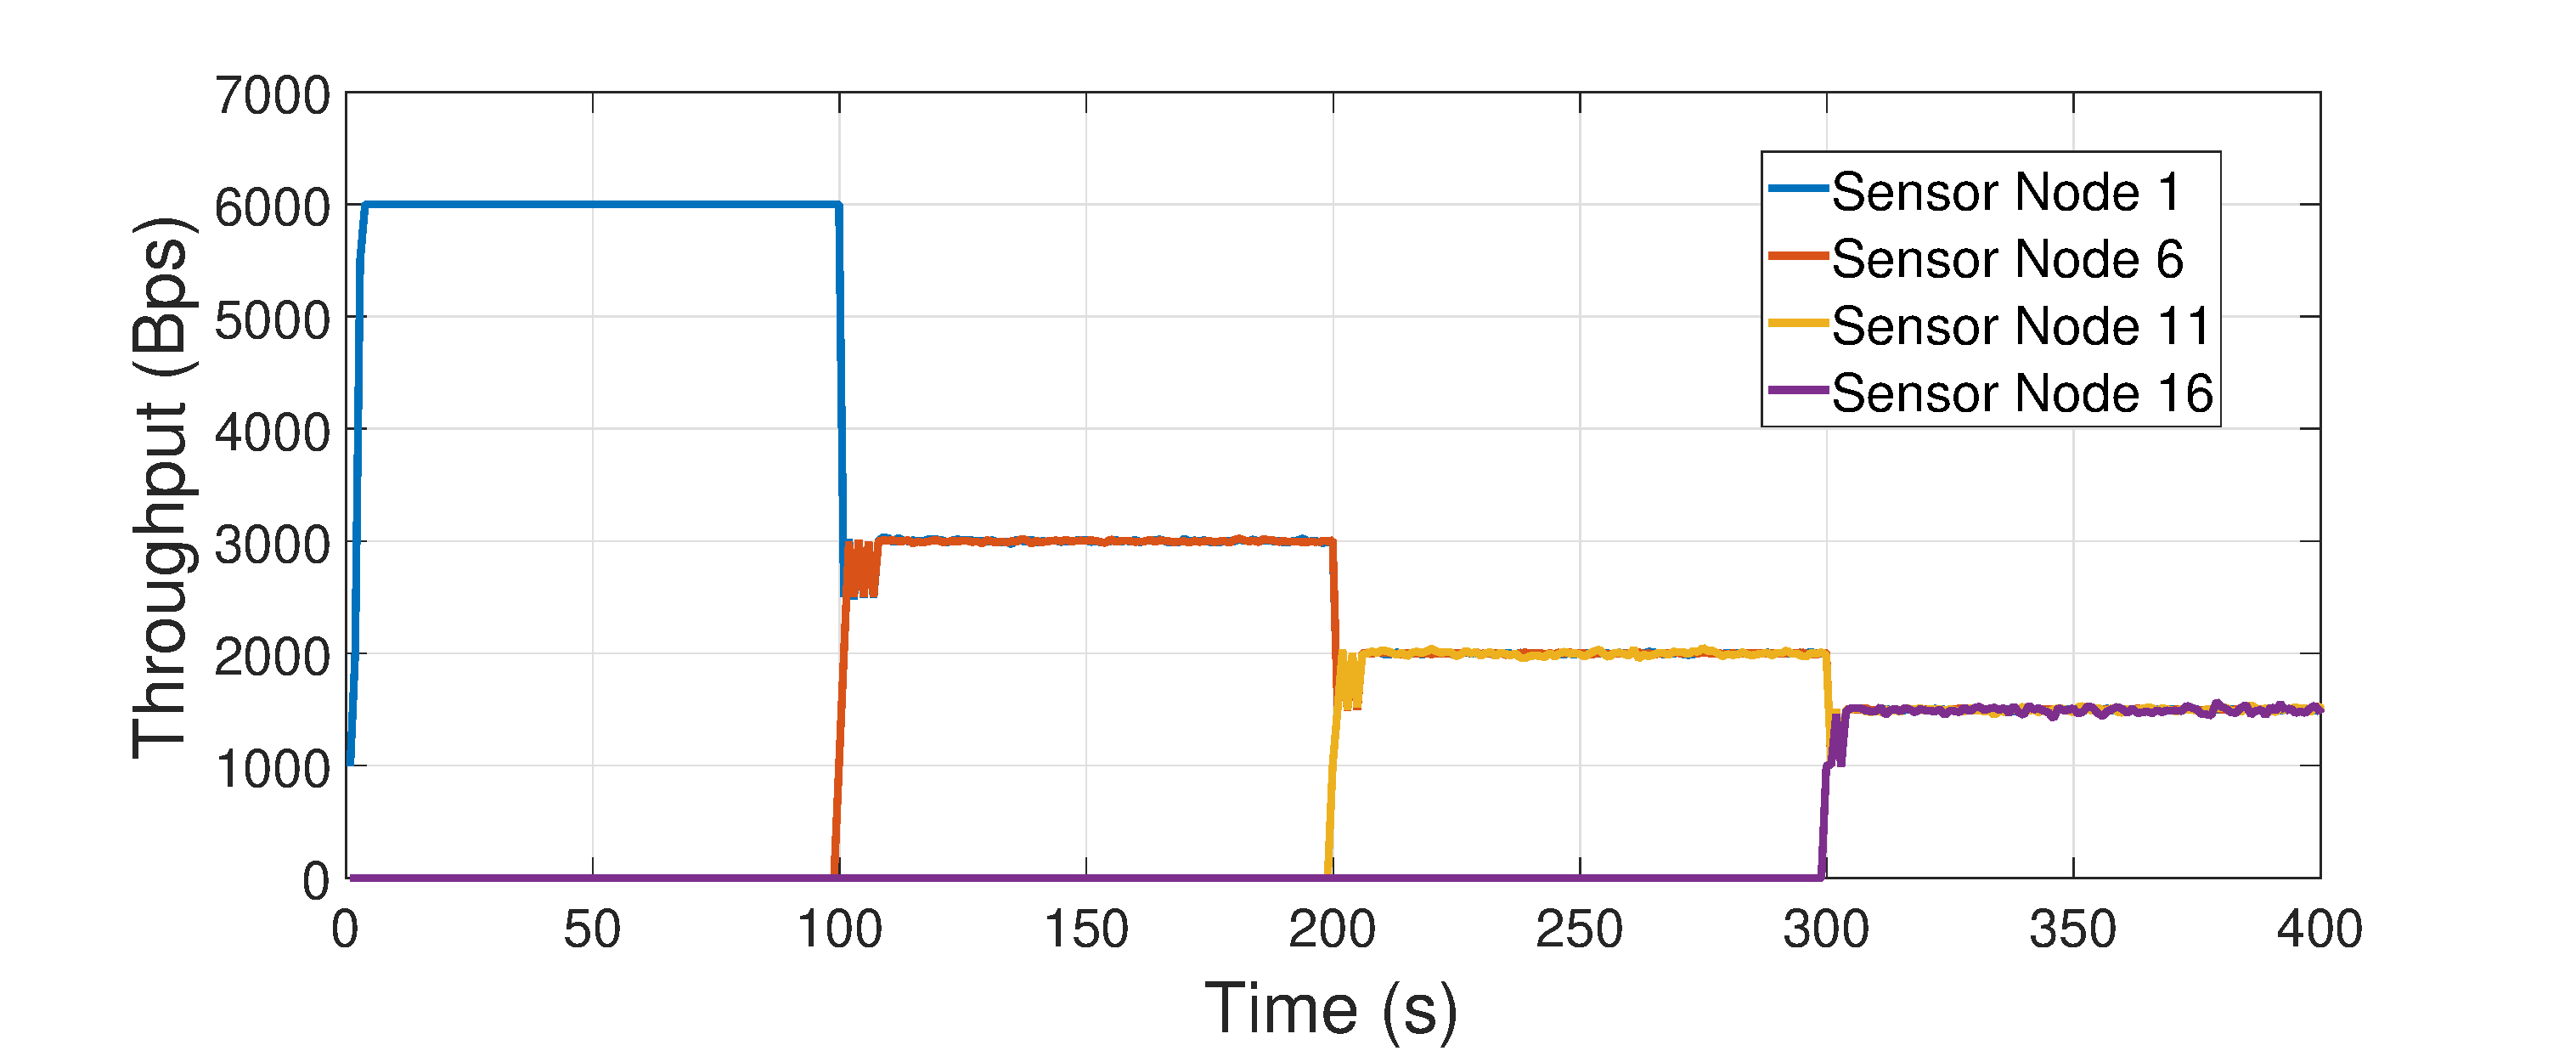
\includegraphics[width=1\linewidth]{pics/LotkaTru}
%	\caption{Throughput with star topology}
%	\label{fig:lotkatru}
%\end{figure}

	\begin{figure}
	\centering
	\begin{subfigure}[b]{0.475\textwidth}
		\centering
		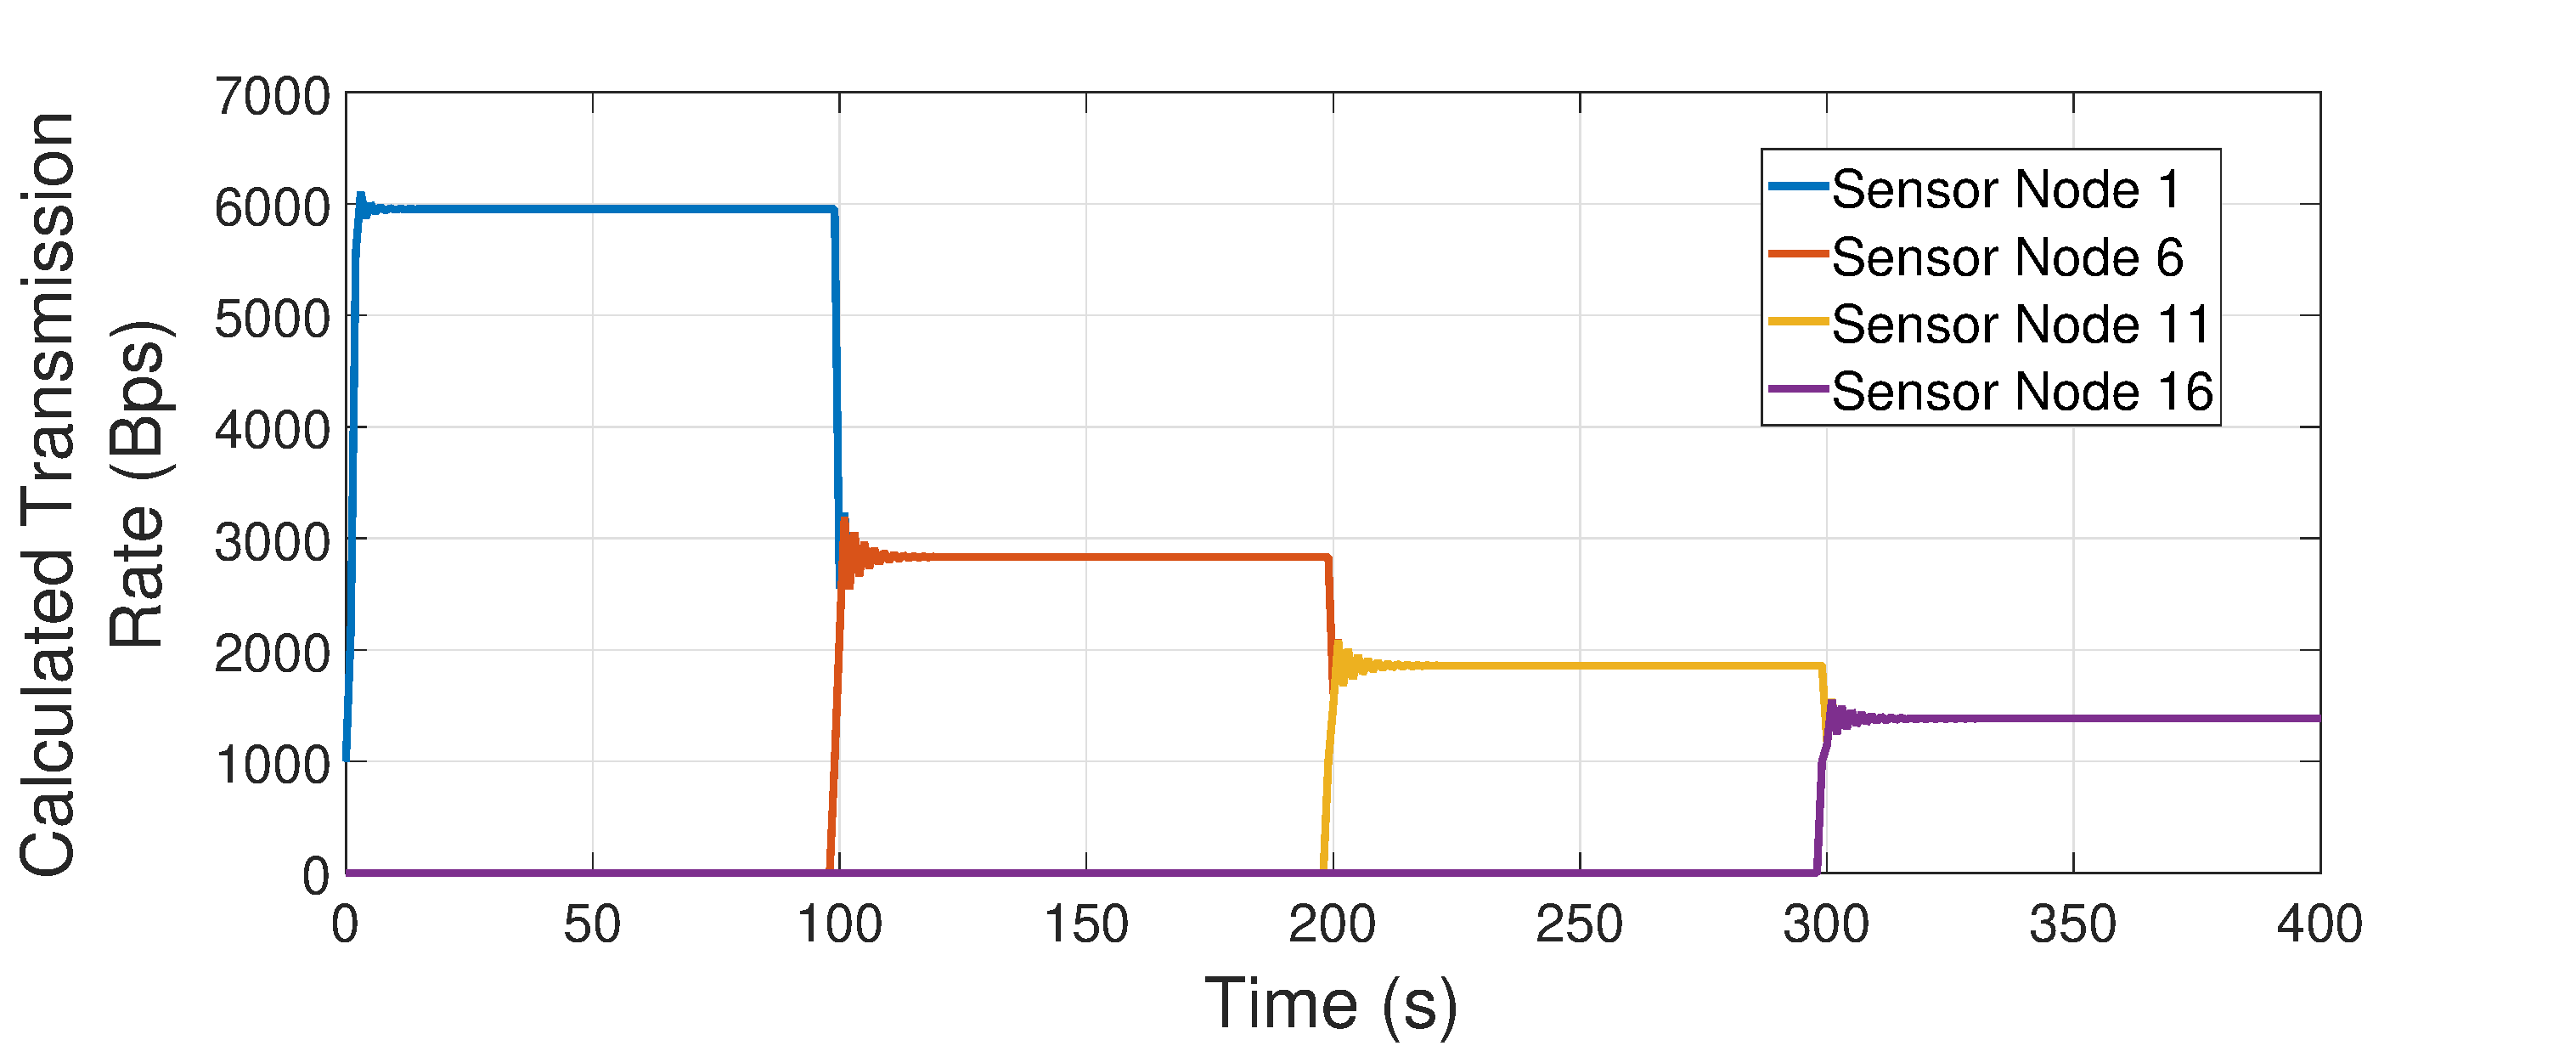
\includegraphics[width=\textwidth, height=0.2\textheight]{pics/Lotka}
		\caption{Transmission Rate with proposed scheme}
		\label{fig:lotka} 
	\end{subfigure}
	\hfill
	\begin{subfigure}[b]{0.475\textwidth}  
		\centering 
		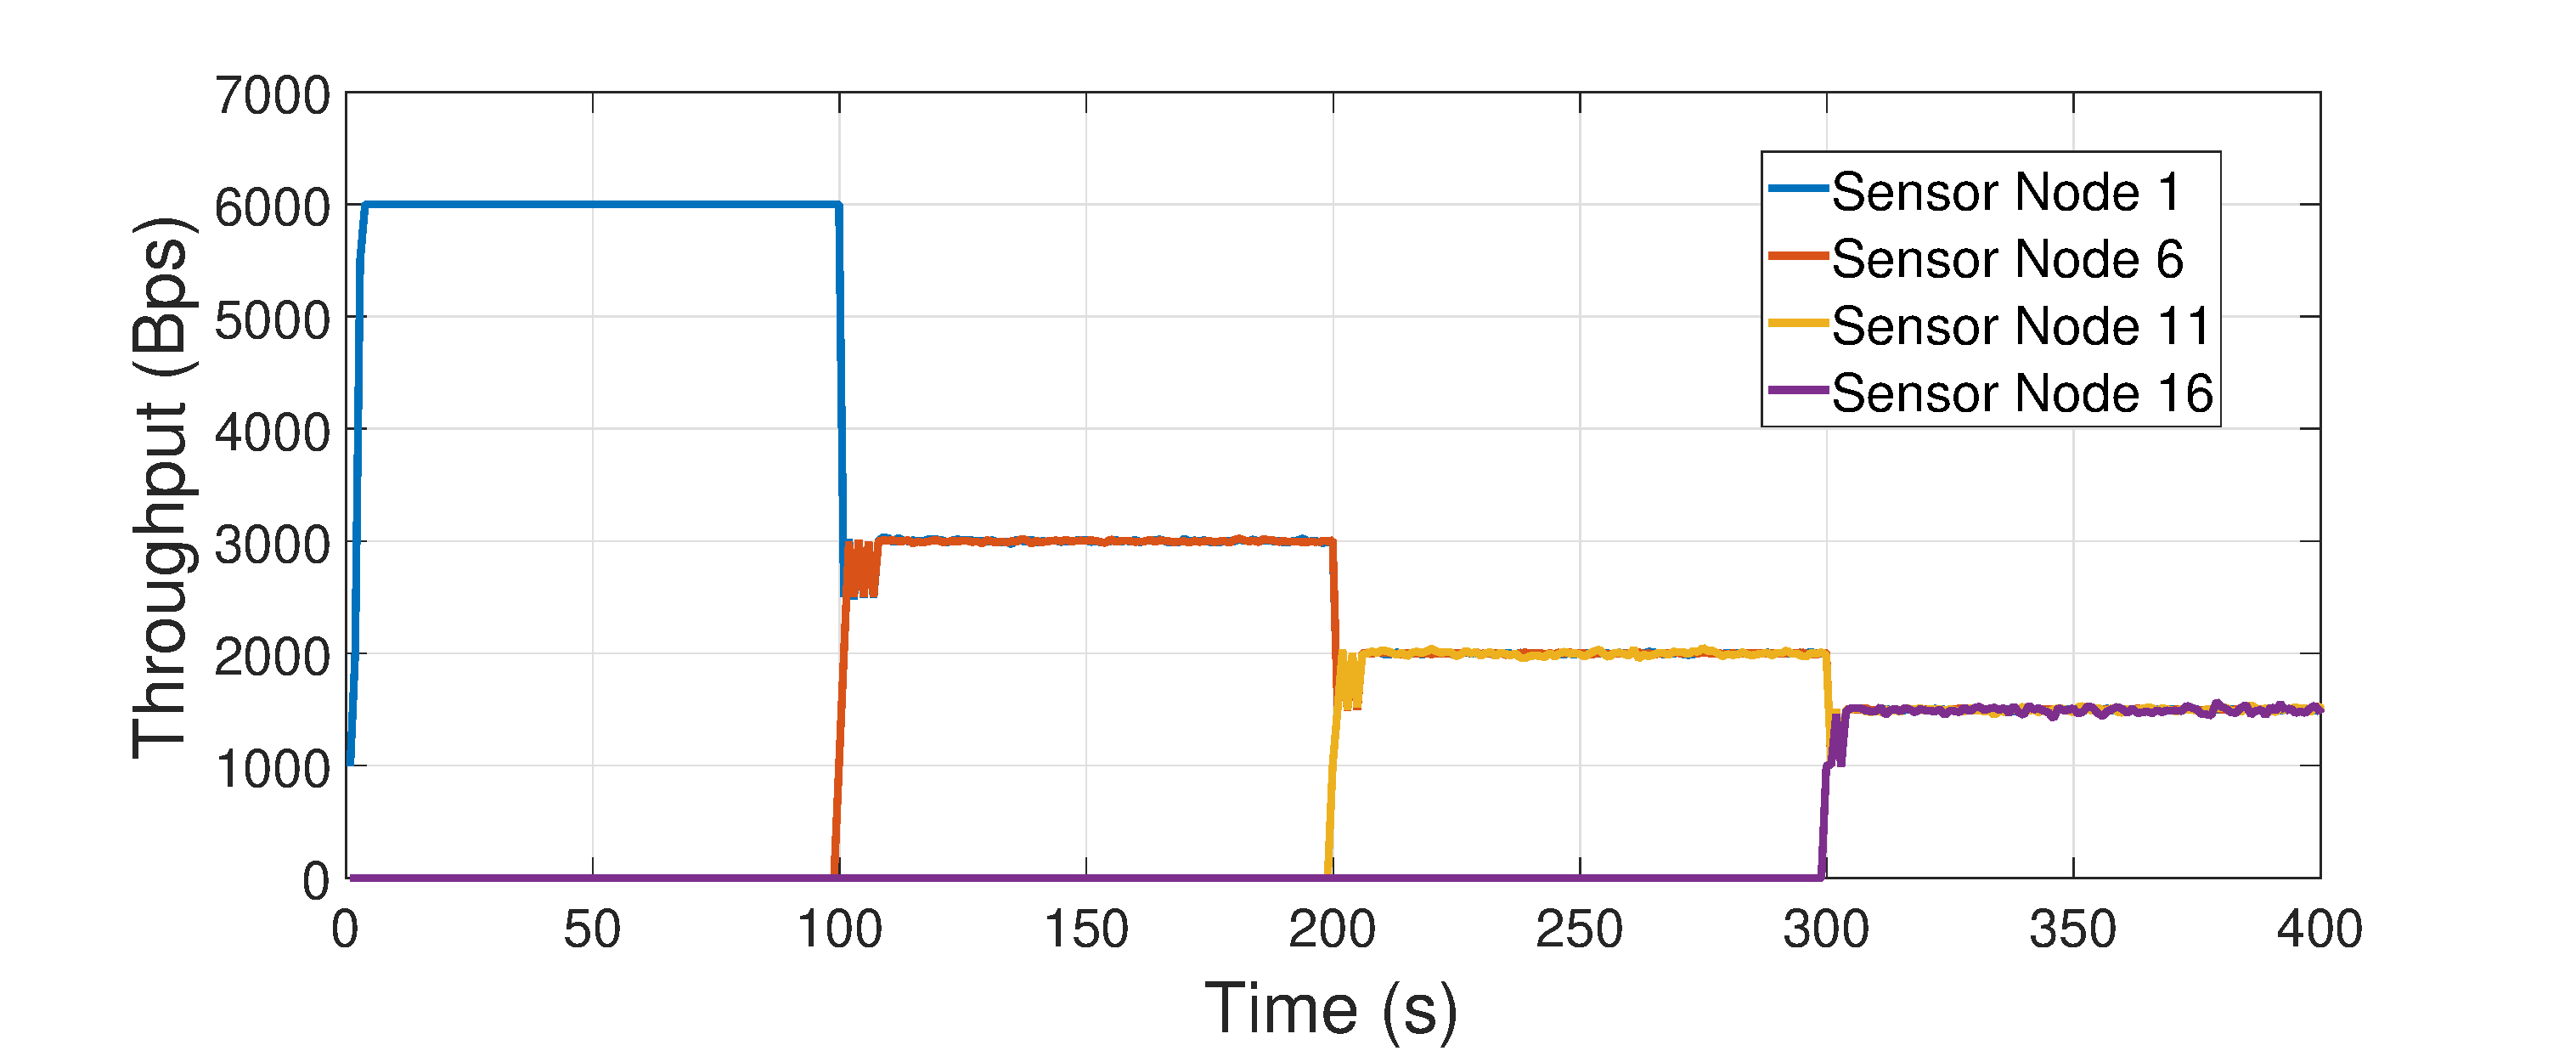
\includegraphics[width=\textwidth, height=0.2\textheight]{pics/LotkaTru}
		\caption{Throughput with proposed scheme}
		\label{fig:lotkatru} % subcaption
	\end{subfigure}
	\vskip\baselineskip
	\begin{subfigure}[b]{0.475\textwidth}   
		\centering 
		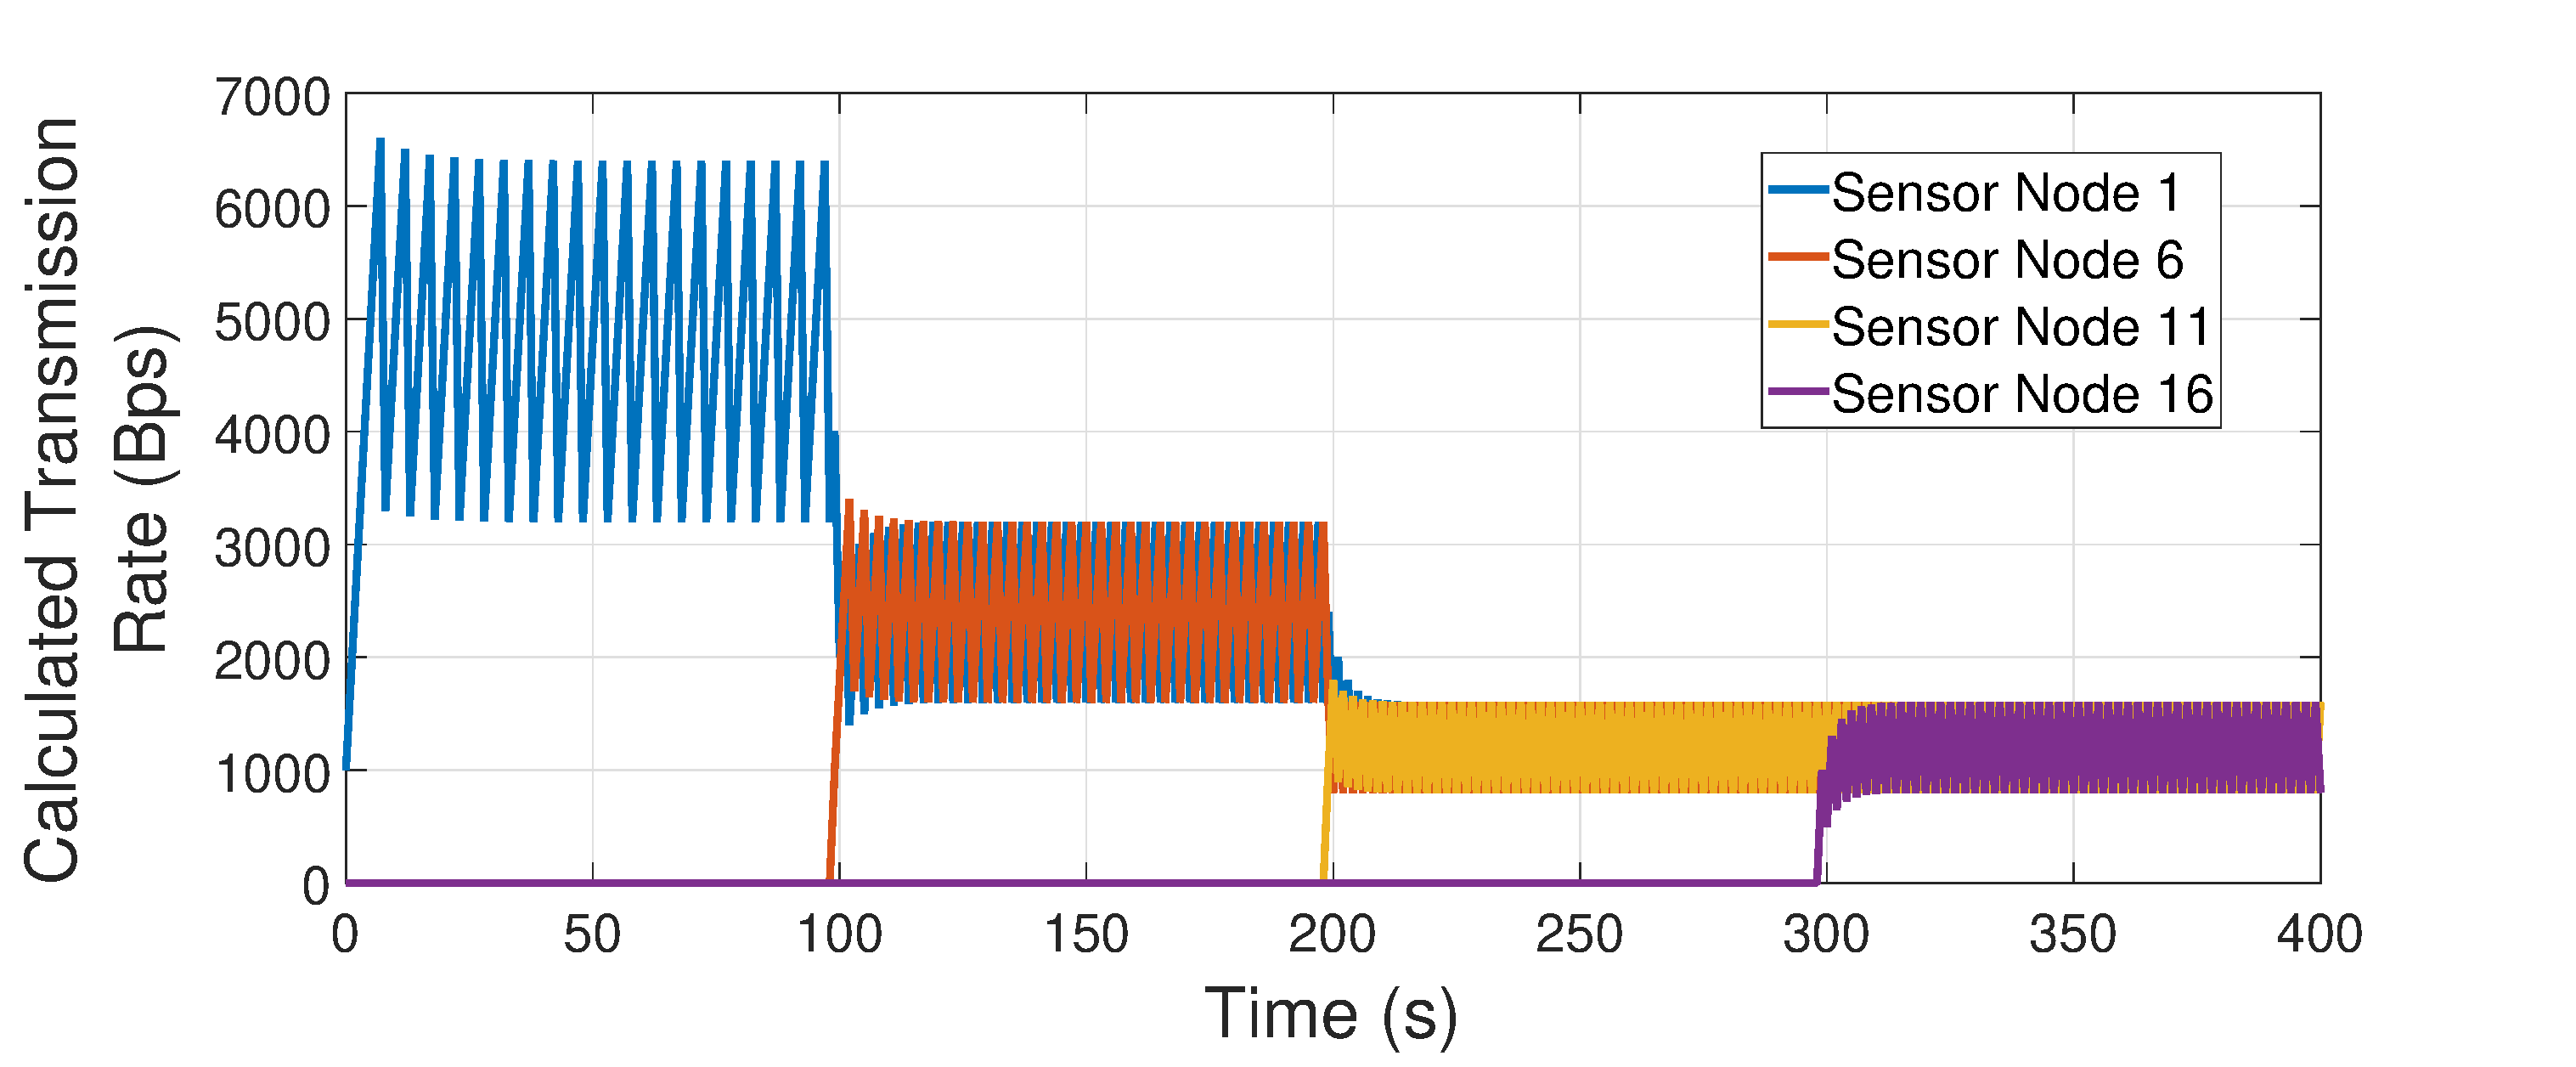
\includegraphics[width=\textwidth, height=0.2\textheight]{pics/AIMD}
		\caption{Transmission Rate with AIMD}
		\label{fig:aimd}
	\end{subfigure}
	\quad
	\begin{subfigure}[b]{0.475\textwidth}   
		\centering 
		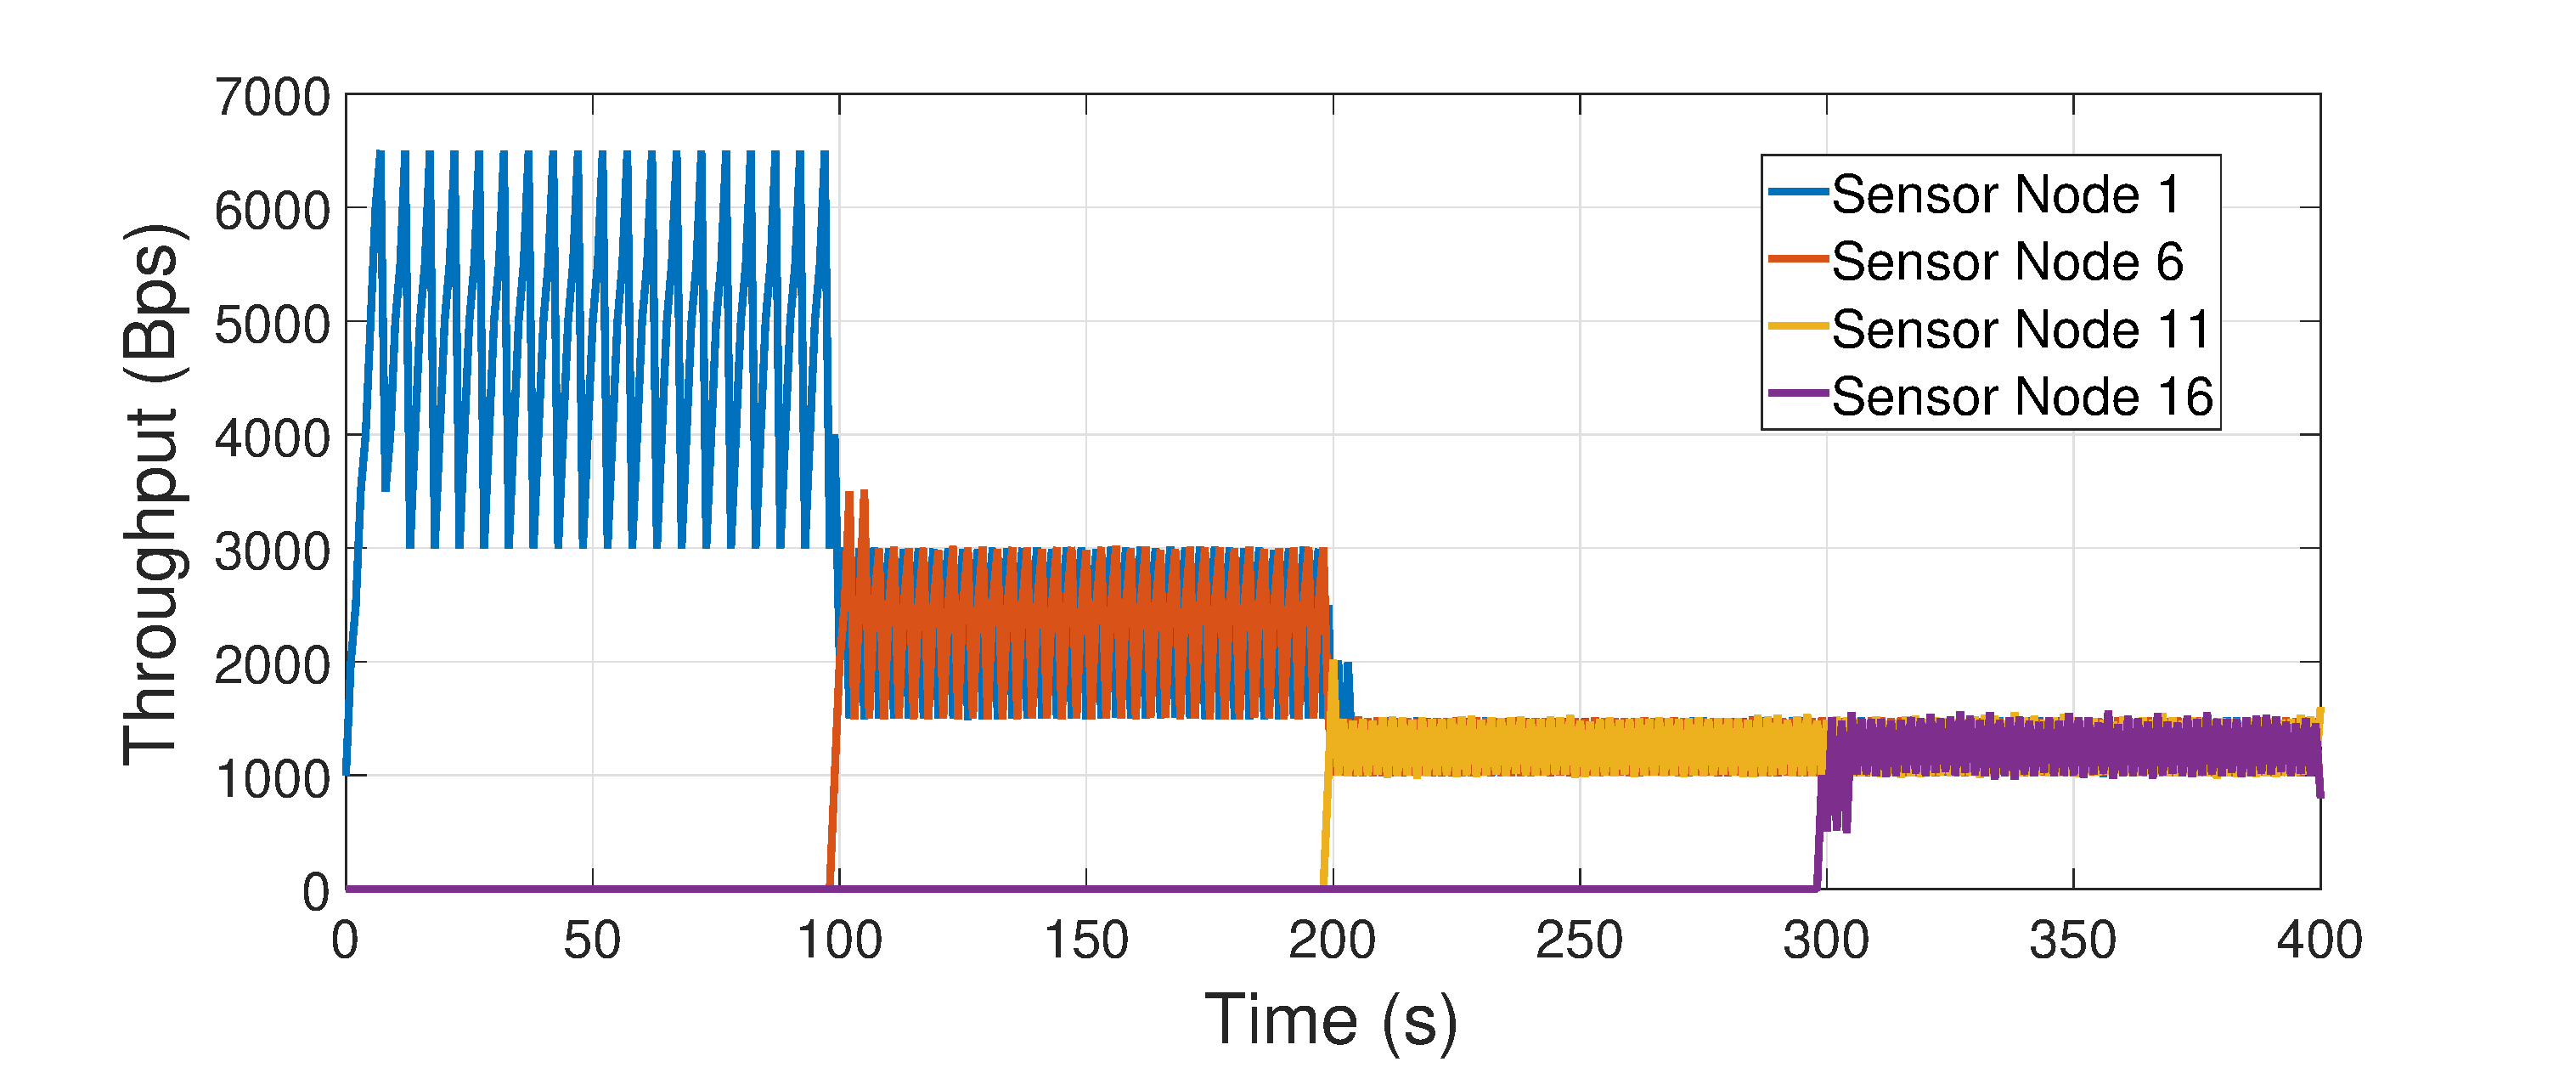
\includegraphics[width=\textwidth, height=0.2\textheight]{pics/AIMDtru}
		\caption{Throughput with AIMD}
		\label{fig:aimdtru}
	\end{subfigure}
	\caption{Transmission Rate and throughput in star topology}  
	\label{fig:gambar}
\end{figure}

\begin{figure}
	\centering
	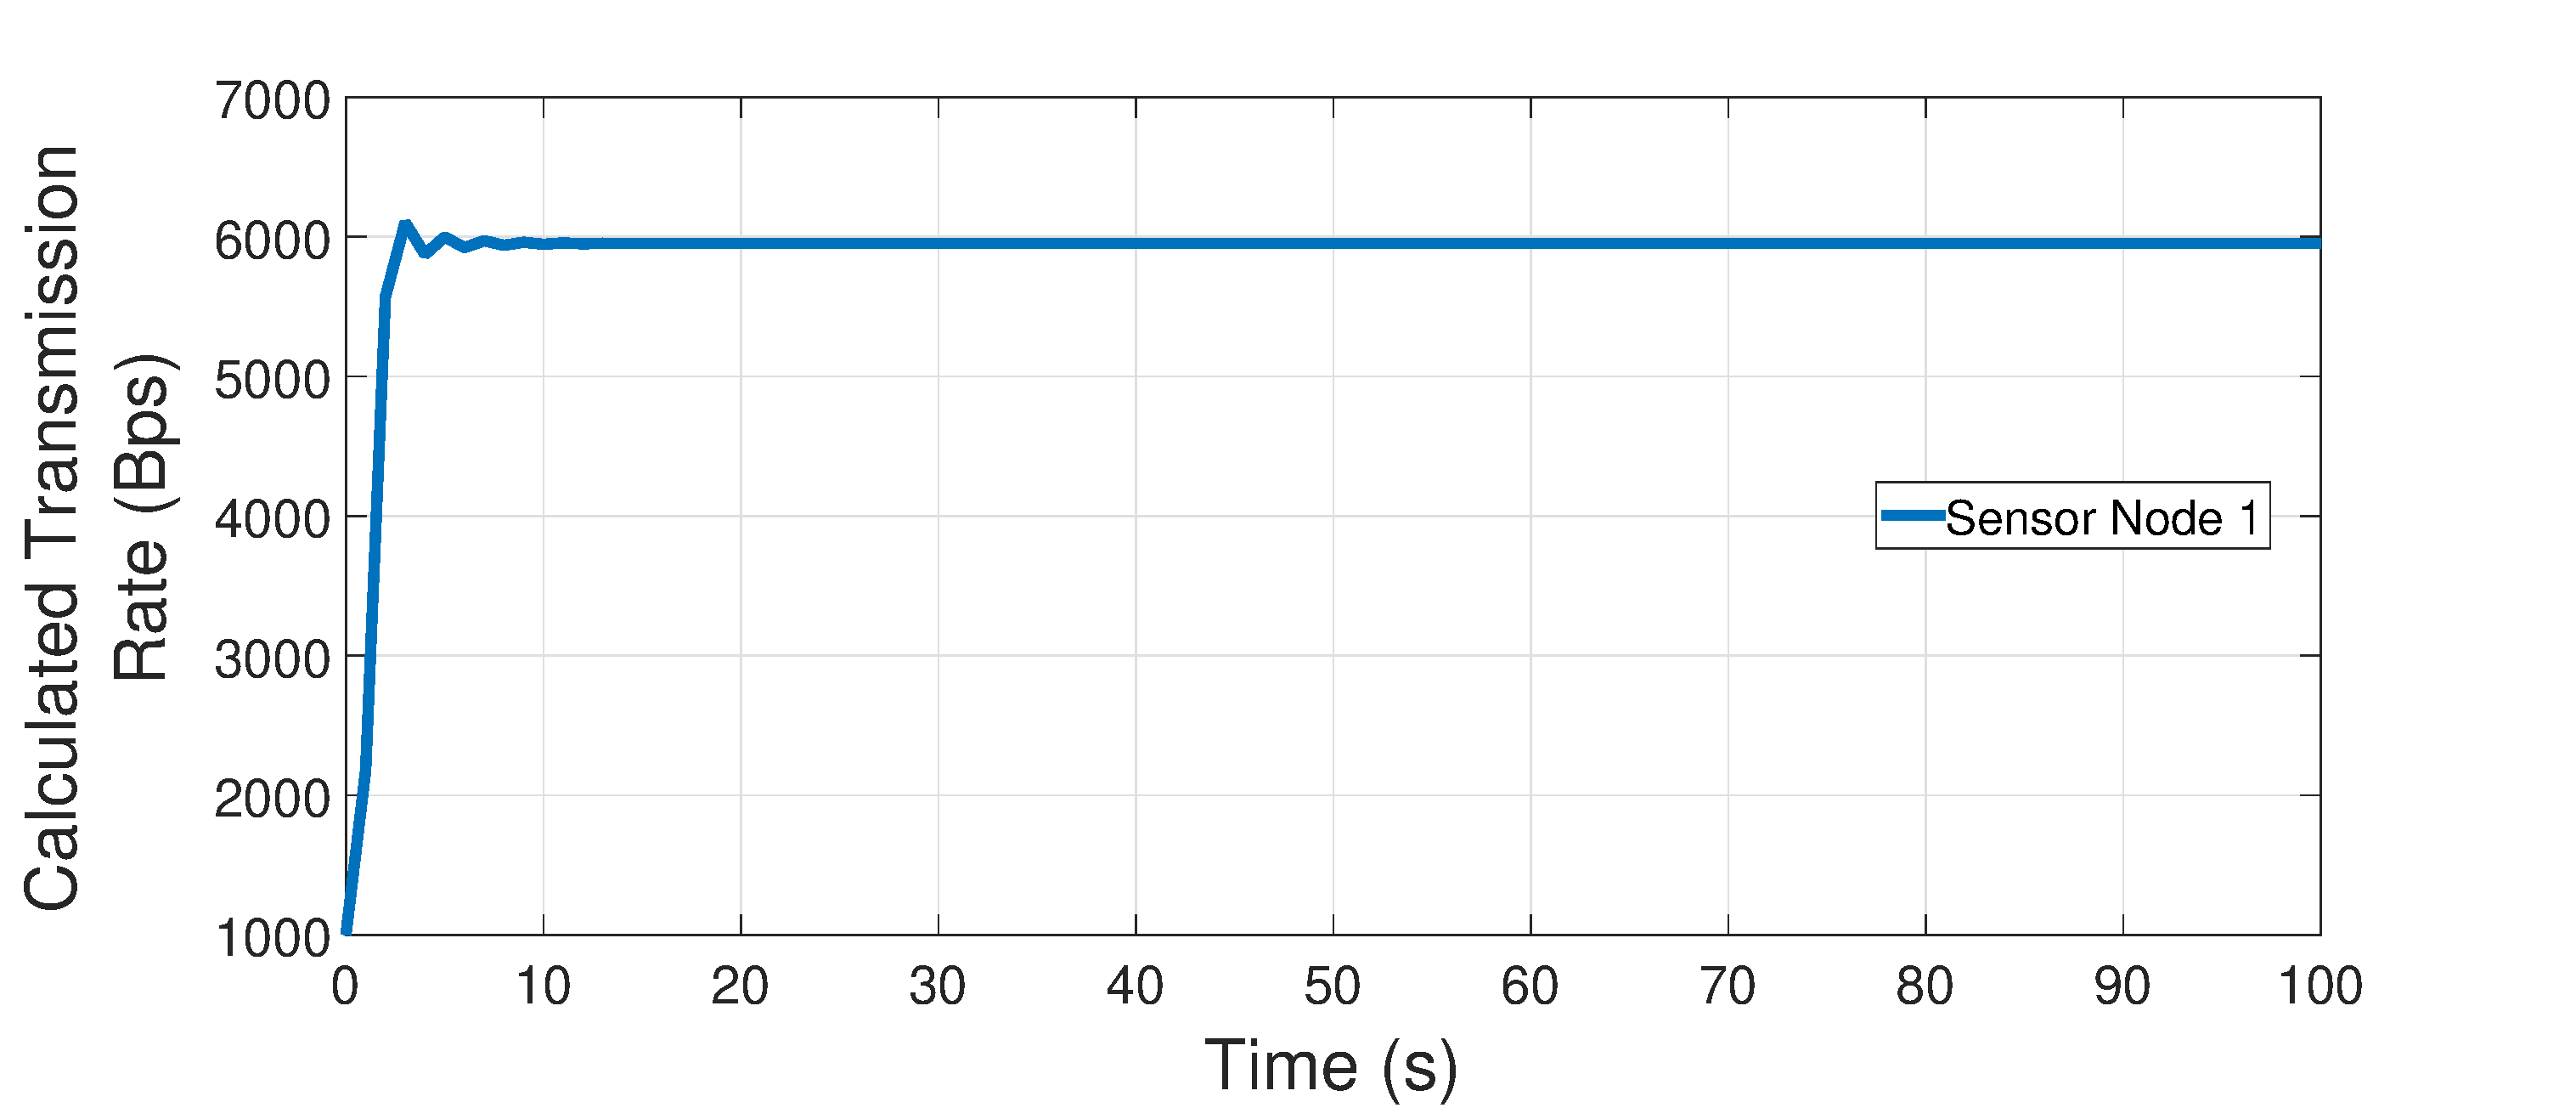
\includegraphics[width=1\linewidth]{pics/Lotka1}
	\caption{Transmission Rate with 5 Nodes Active}
	\label{fig:lotka1}
\end{figure}

\begin{figure}
	\centering
	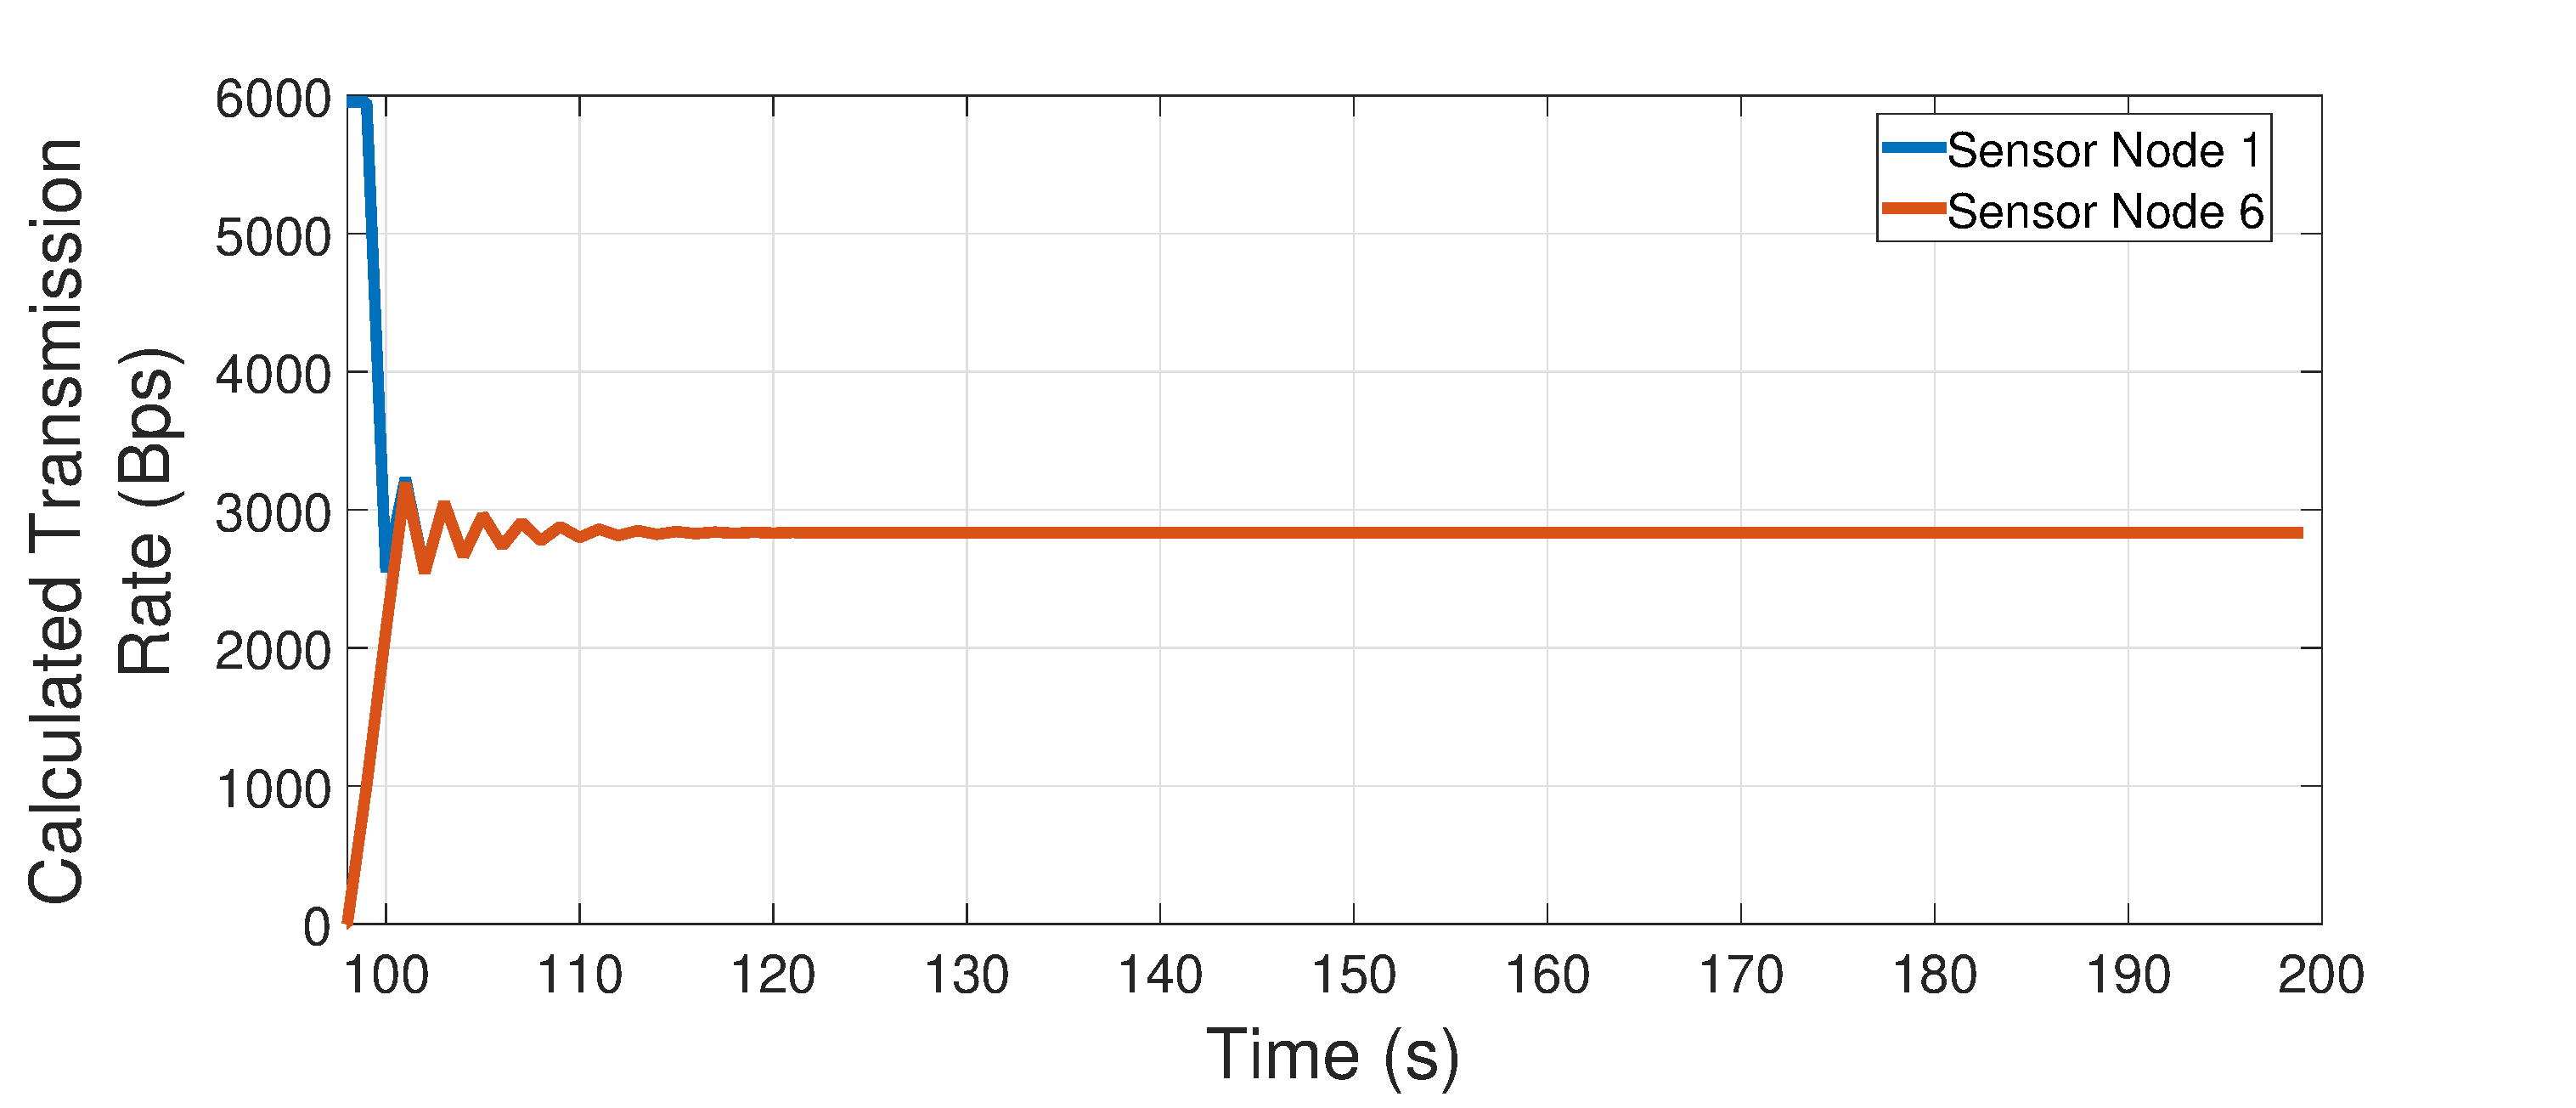
\includegraphics[width=1\linewidth]{pics/Lotka2}
	\caption{Transmission Rate with 10 Nodes Active}
	\label{fig:lotka2}
\end{figure}

\begin{figure}
	\centering
	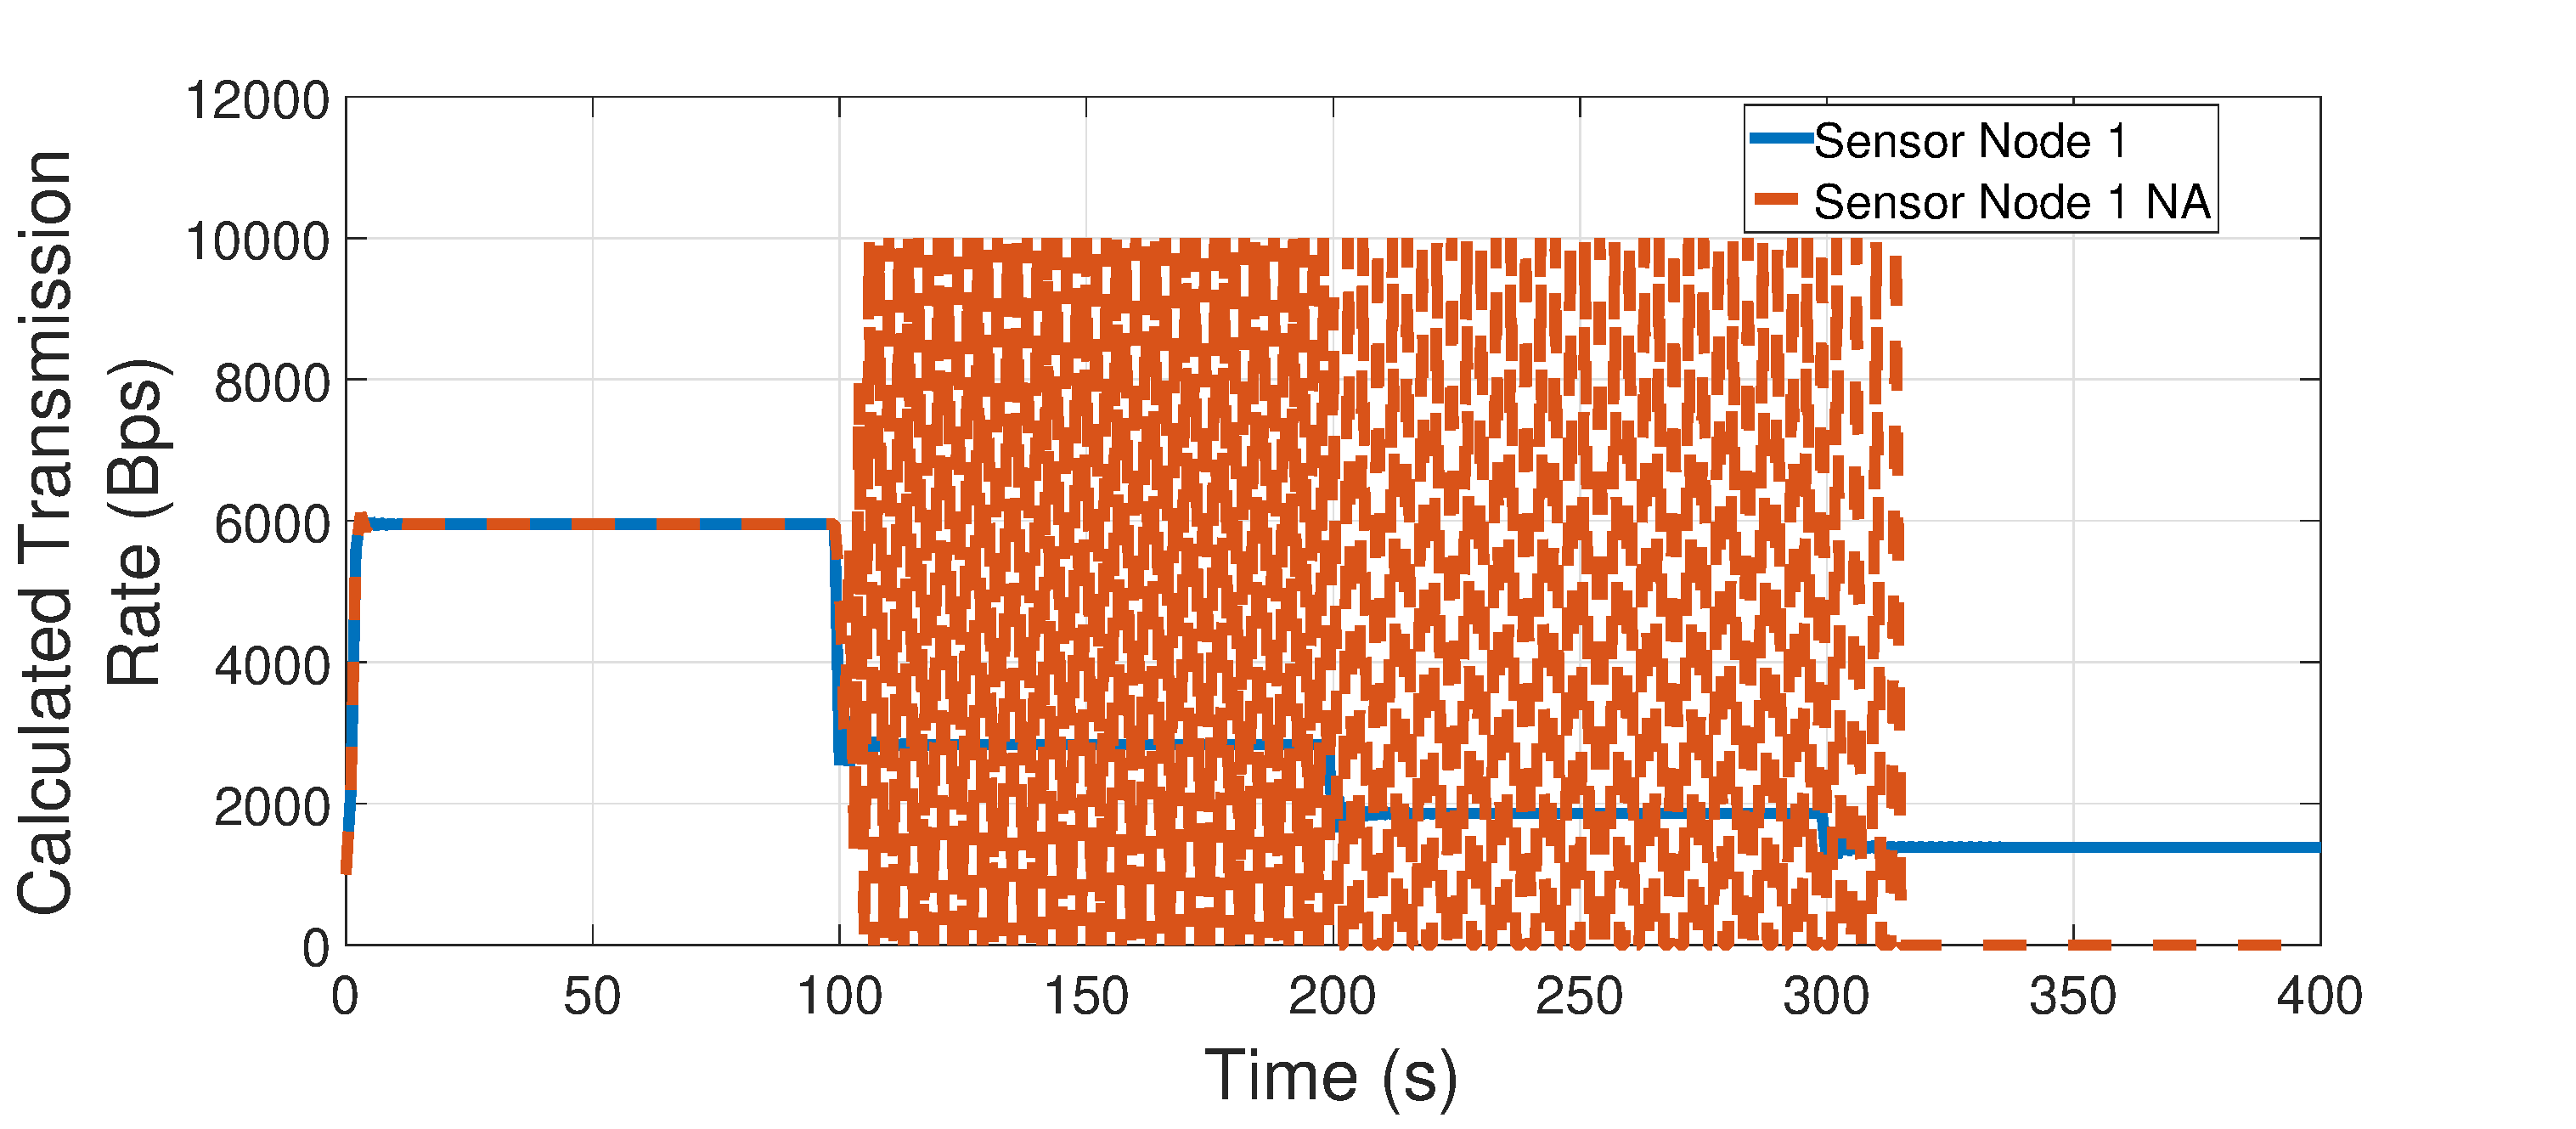
\includegraphics[width=1\linewidth]{pics/comp1}
	\caption{Compared with Non-Adaptive Scheme of C-LV}
	\label{fig:comp1}
\end{figure}

The proposed scheme was compared with conventional AIMD rate adaptation for congestion avoidance. As shown in Fig. \ref{fig:lotka} and Fig. \ref{fig:lotkatru}, the proposed scheme obtained stable and smooth throughput while maintaining fairness. This smooth result due to calculated transmission rate which fairly determines the value based on available capacity. On the other hand, as shown in Fig. \ref{fig:aimd} and Fig. \ref{fig:aimdtru}, AIMD scheme shows saw-tooth-like results. This saw-tooth-like result occurs due to multiplicative rate decrease after congestion occurs. Congestion control scheme by AIMD is ineffective in the industrial wireless environment due to harsh condition and frequent packet loss. Furthermore, it leads to high delay and high error rates.

%\begin{figure}
%	\centering
%	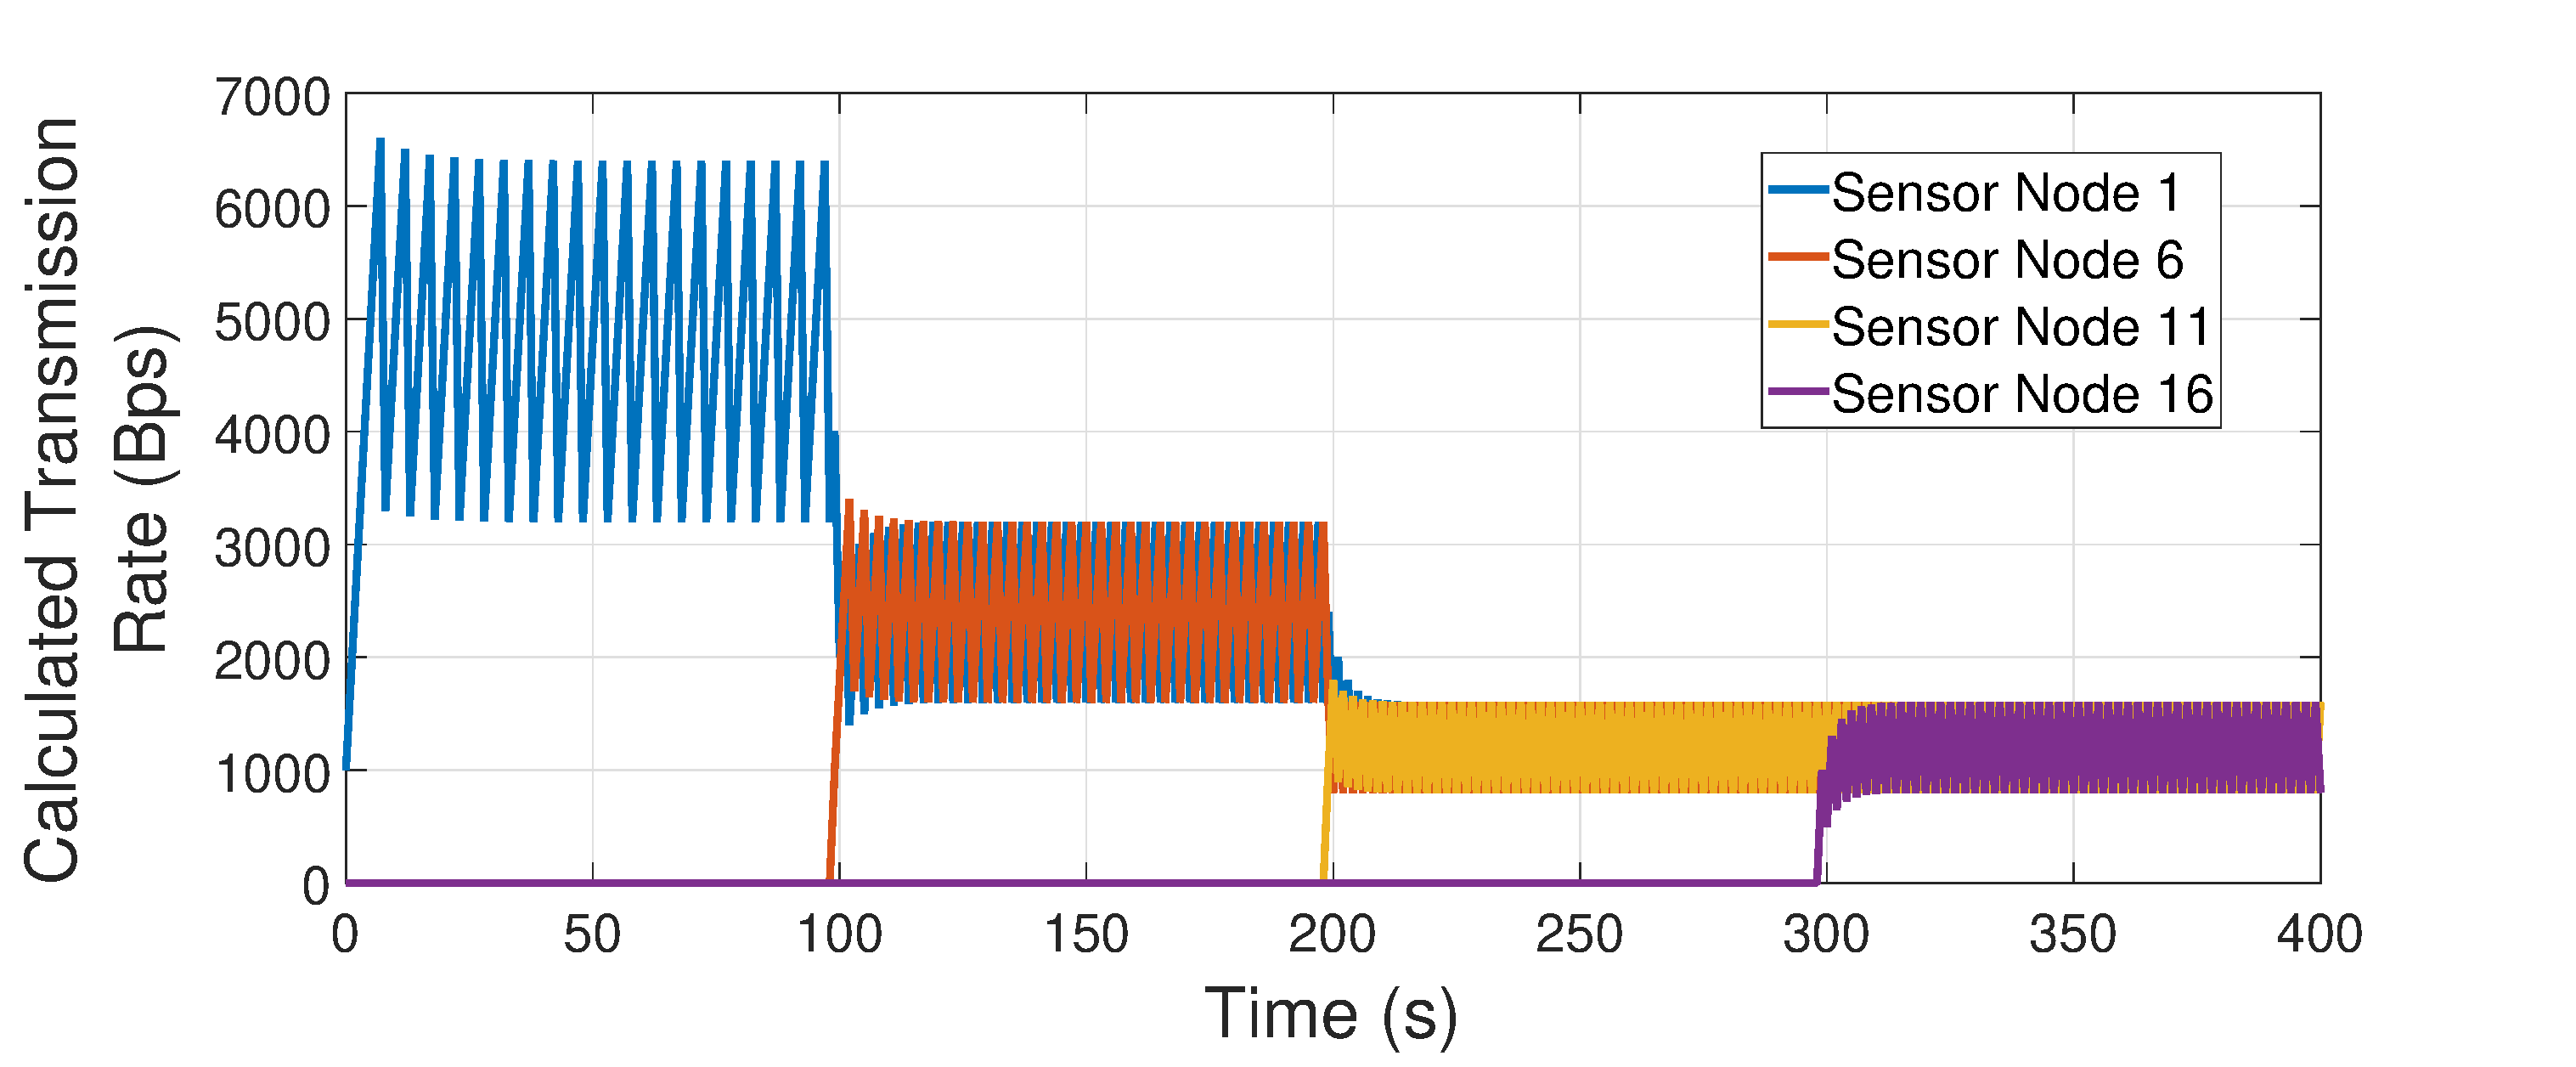
\includegraphics[width=1\linewidth]{pics/AIMD}
%	\caption{Calculated Transmission Rate with AIMD}
%	\label{fig:aimd}
%\end{figure}
%
%\begin{figure}
%	\centering
%	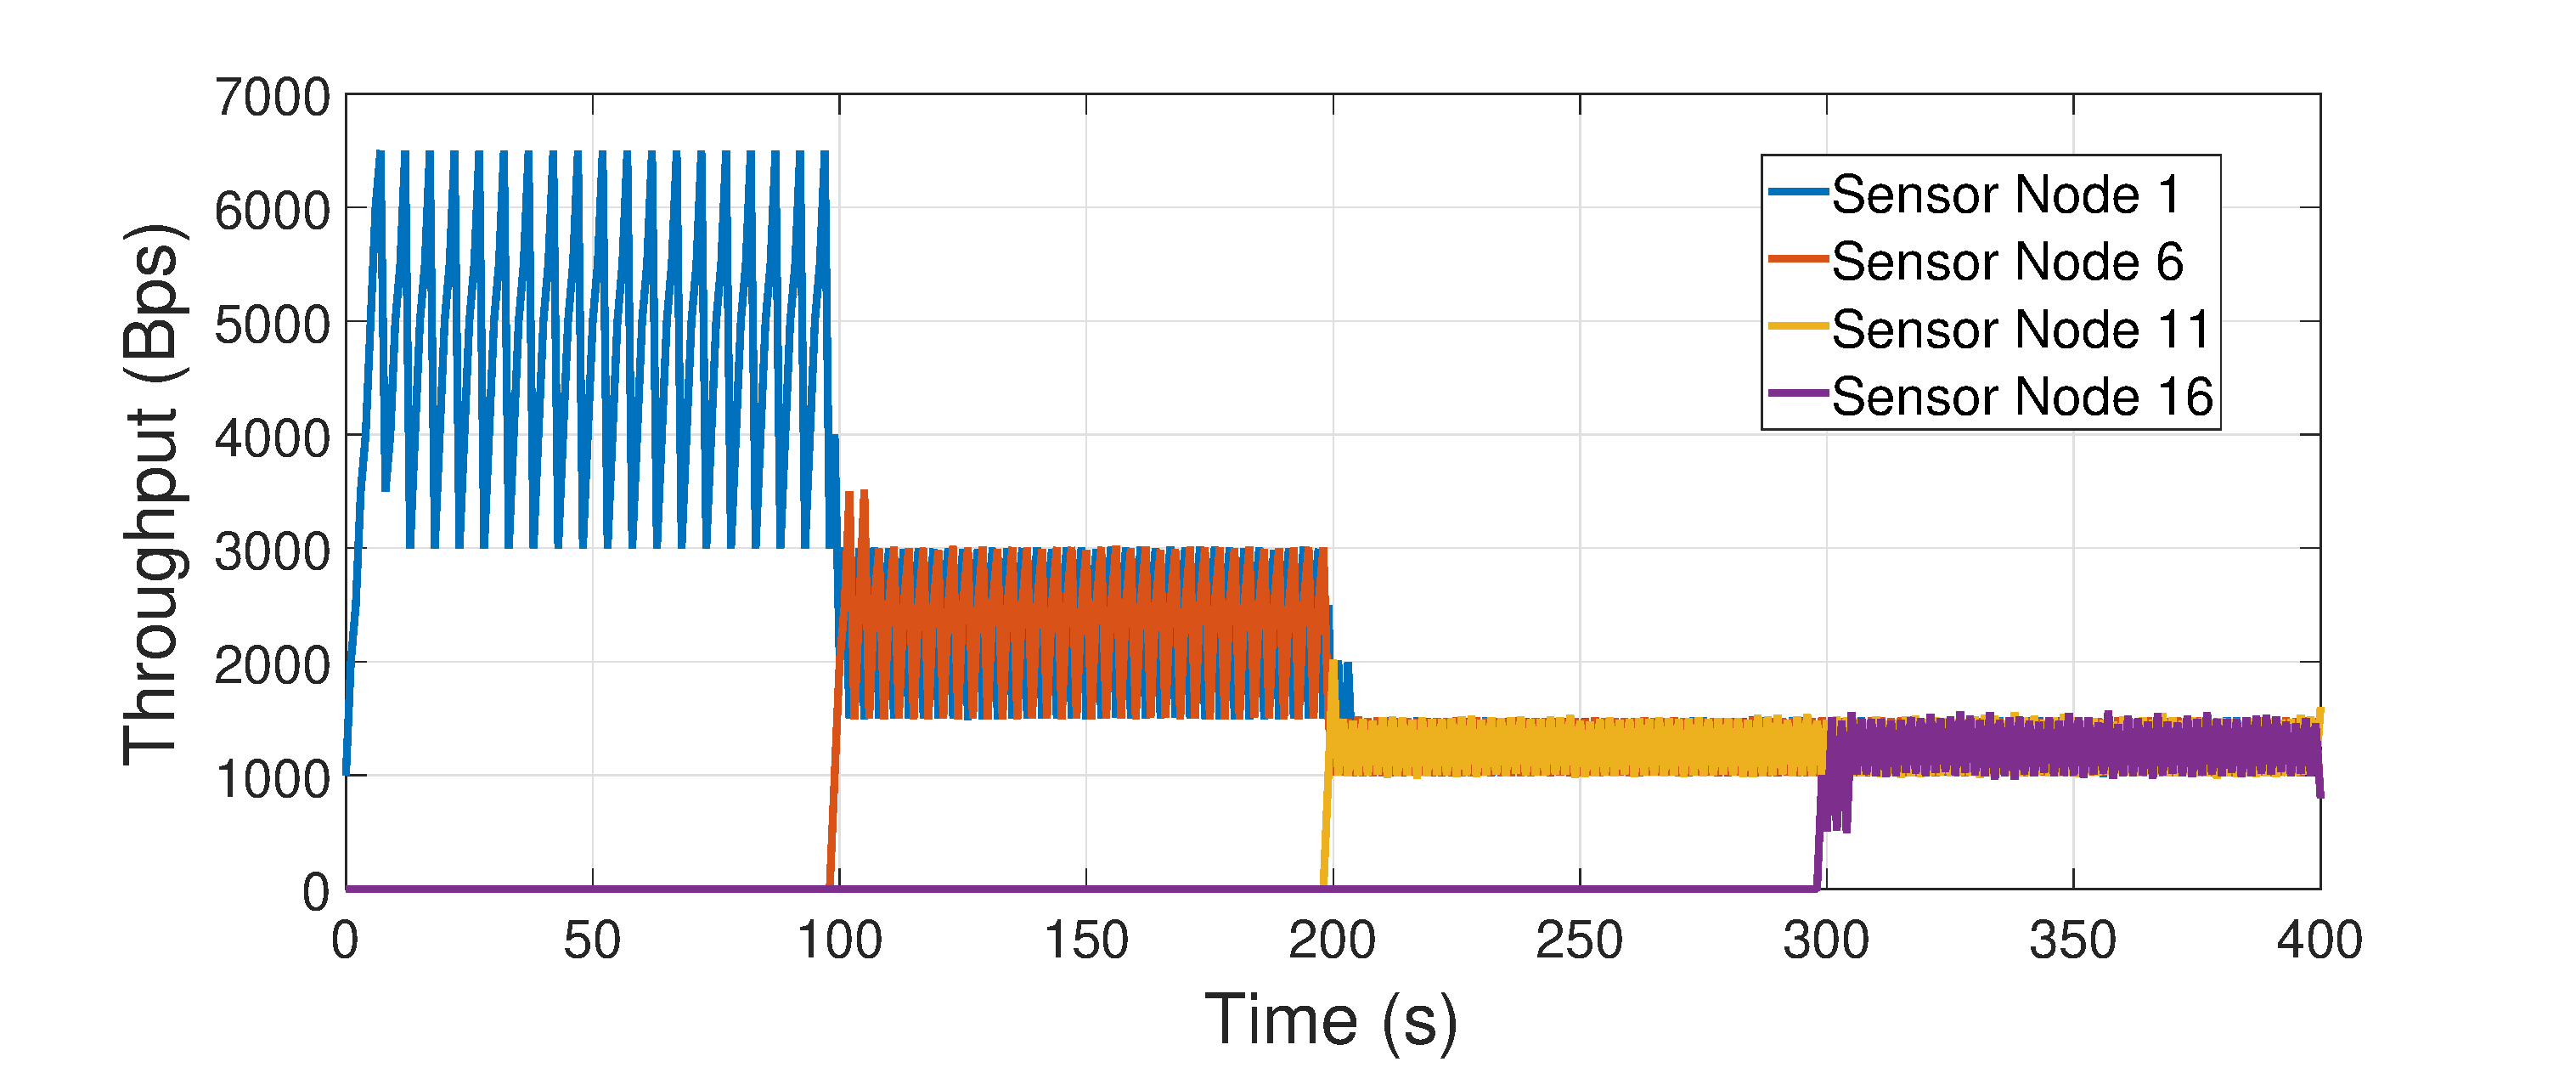
\includegraphics[width=1\linewidth]{pics/AIMDtru}
%	\caption{Throughput with AIMD}
%	\label{fig:aimdtru}
%\end{figure}

\subsection{Simulation Result With Mesh Topology}

In the second scenario, mesh topology shown in Fig. \ref{fig:kuda} was investigated. In this scenario, the calculated transmission rate from a sensor node to cluster head is determined by Eq. \ref{horse}, and the calculated transmission rate from cluster head to the sink node is determined by Eq. \ref{horseliar}.
As shown in Fig. \ref{fig:mesh}, the proposed scheme show a good result. The throughput is still stable when a number of nodes increased even rough noise exists due to interference. This result also shows that this scheme can be scalable and can be applied topology with predefined routing path.	

\begin{figure}
	\centering
	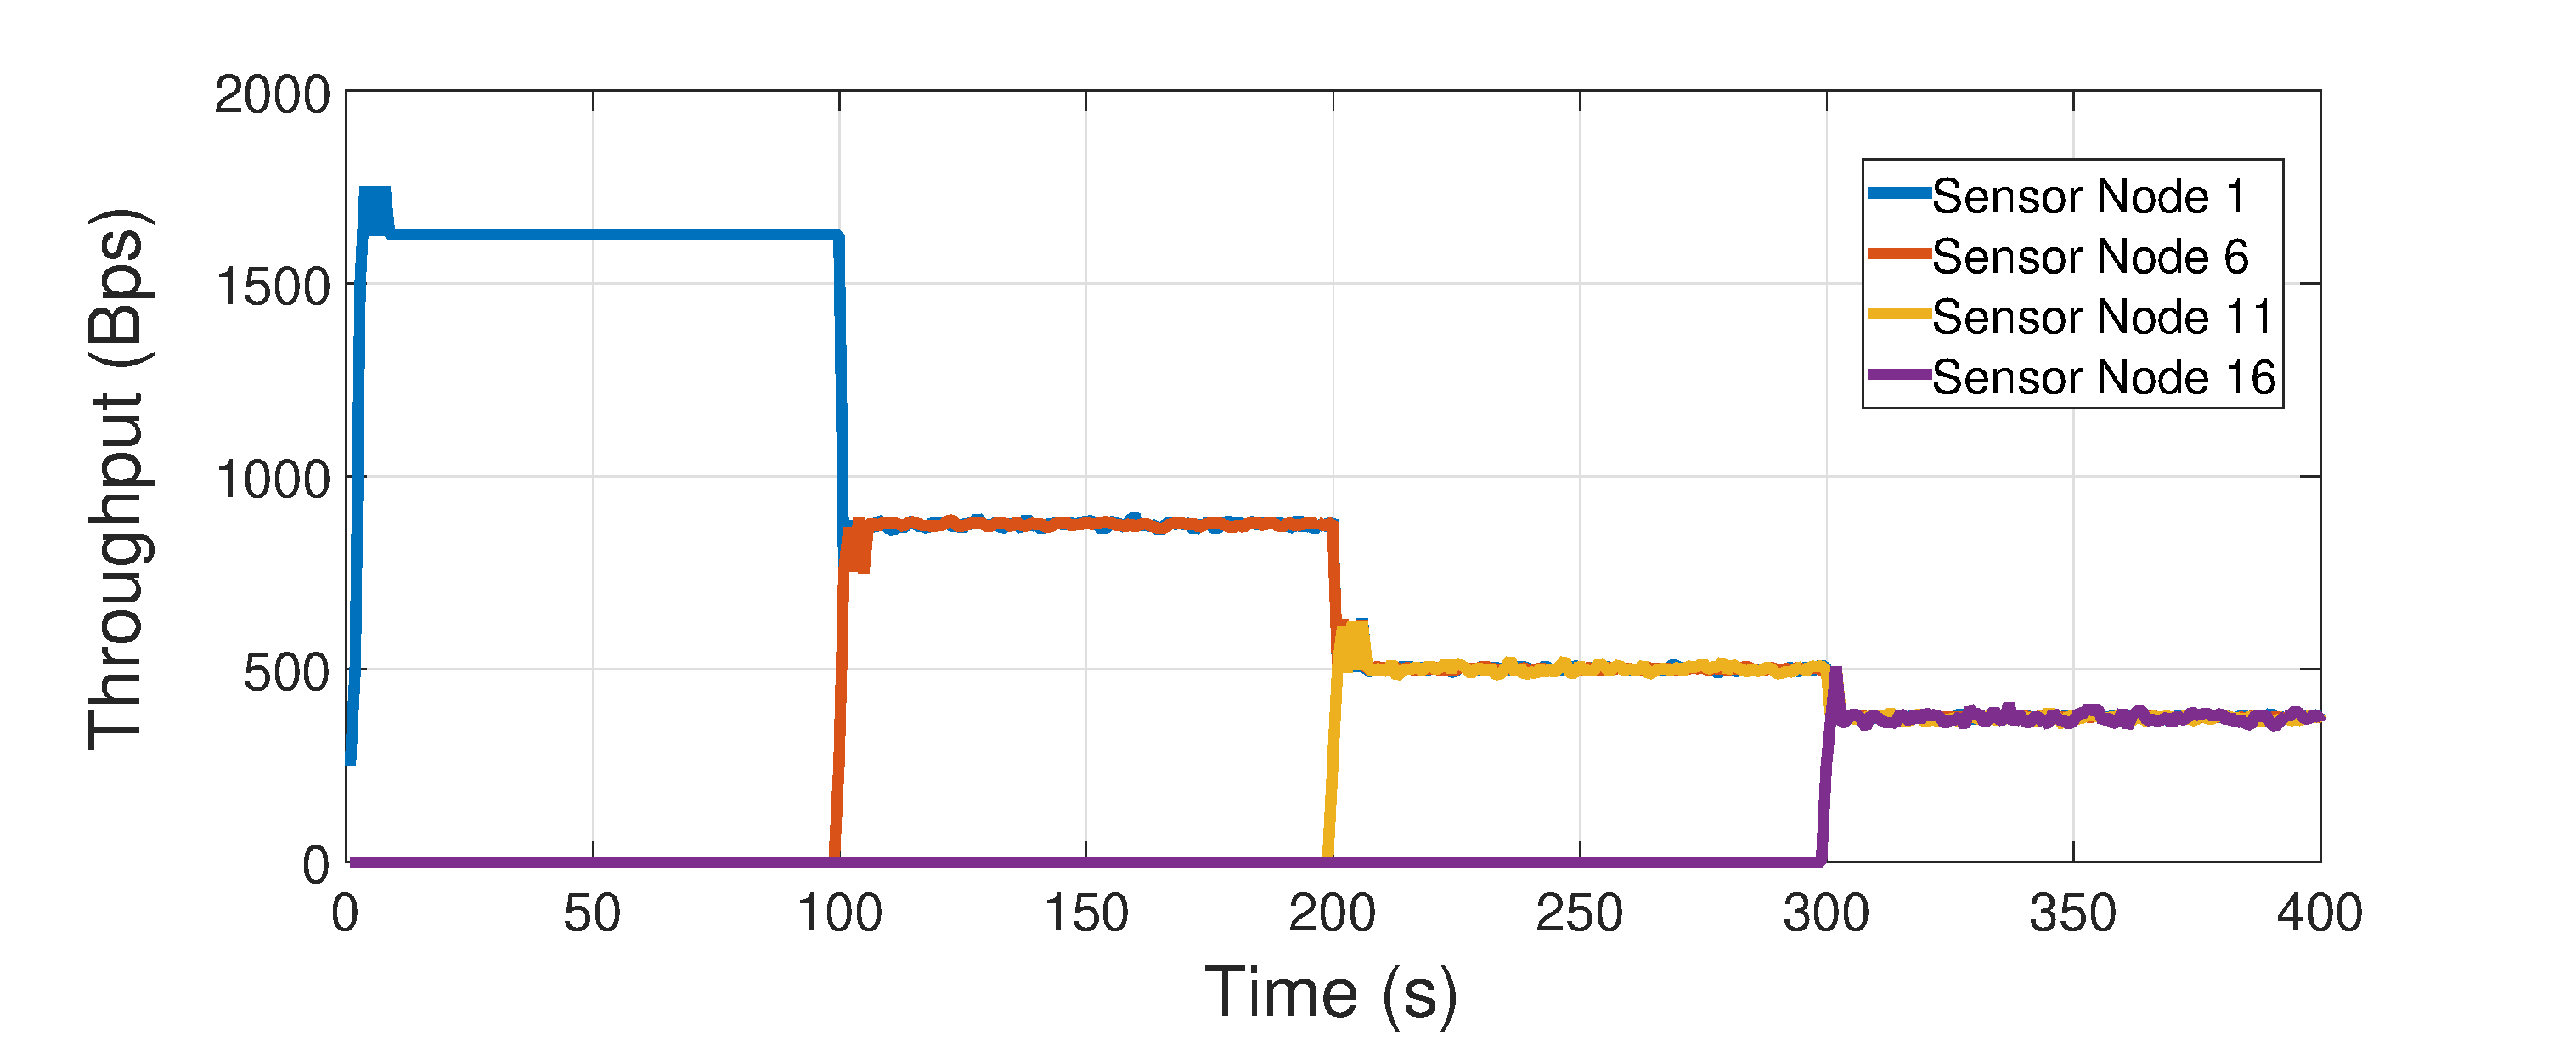
\includegraphics[width=1\linewidth]{pics/mesh}
	\caption{Throughput with mesh topology.}
	\label{fig:mesh}
\end{figure}

\subsection{Simulation Result With Different Priority}

To make different priority classes, $\alpha_{ij}$ has different values for each priority. For instance, in this work, three priority classes were considered. The three priority classes are high, medium, and low.  Without loss of generality, it is assumed that $\{1,2,..,p\} \in \mathbf{H}$, $\{p+1,p+2,..,q\} \in \mathbf{M}$, and $\{q+1,q+2,..,n\} \in \mathbf{L}$, with $p<q<n$. Additionally, $\mathbf{H}$, $\mathbf{M}$, and $\mathbf{L}$ are sets of species with high, medium, and low priority class respectively. Therefore, it can be concluded that
\begin{align}
	\begin{split}
		&\forall i \in \mathbf{H},~a_{i}=a_H, \\
		&\forall i \in \mathbf{M},~a_{i}=a_M,~~~~\text{with}~~a_H>a_M>a_L\\
		&\forall i \in \mathbf{L},~a_{i}=a_L. 
	\end{split}
\end{align}

In this thesis, evaluation of proposed method with different priority was investigated with star topology. And simulation was conducted with the same scenario that was conducted in star topology section. In this evaluation, $\{SN1, SN6, SN11, SN16\} \in \textbf{H}$, $\{SN2, SN7, SN12, SN17\} \in \textbf{M}$, and the rest has low priority. As shown in Fig. \ref{fig:comp2}, the proposed scheme works well with different priority. Therefore time-critical data can be prioritized in this proposed scheme.

\begin{figure}
	\centering
	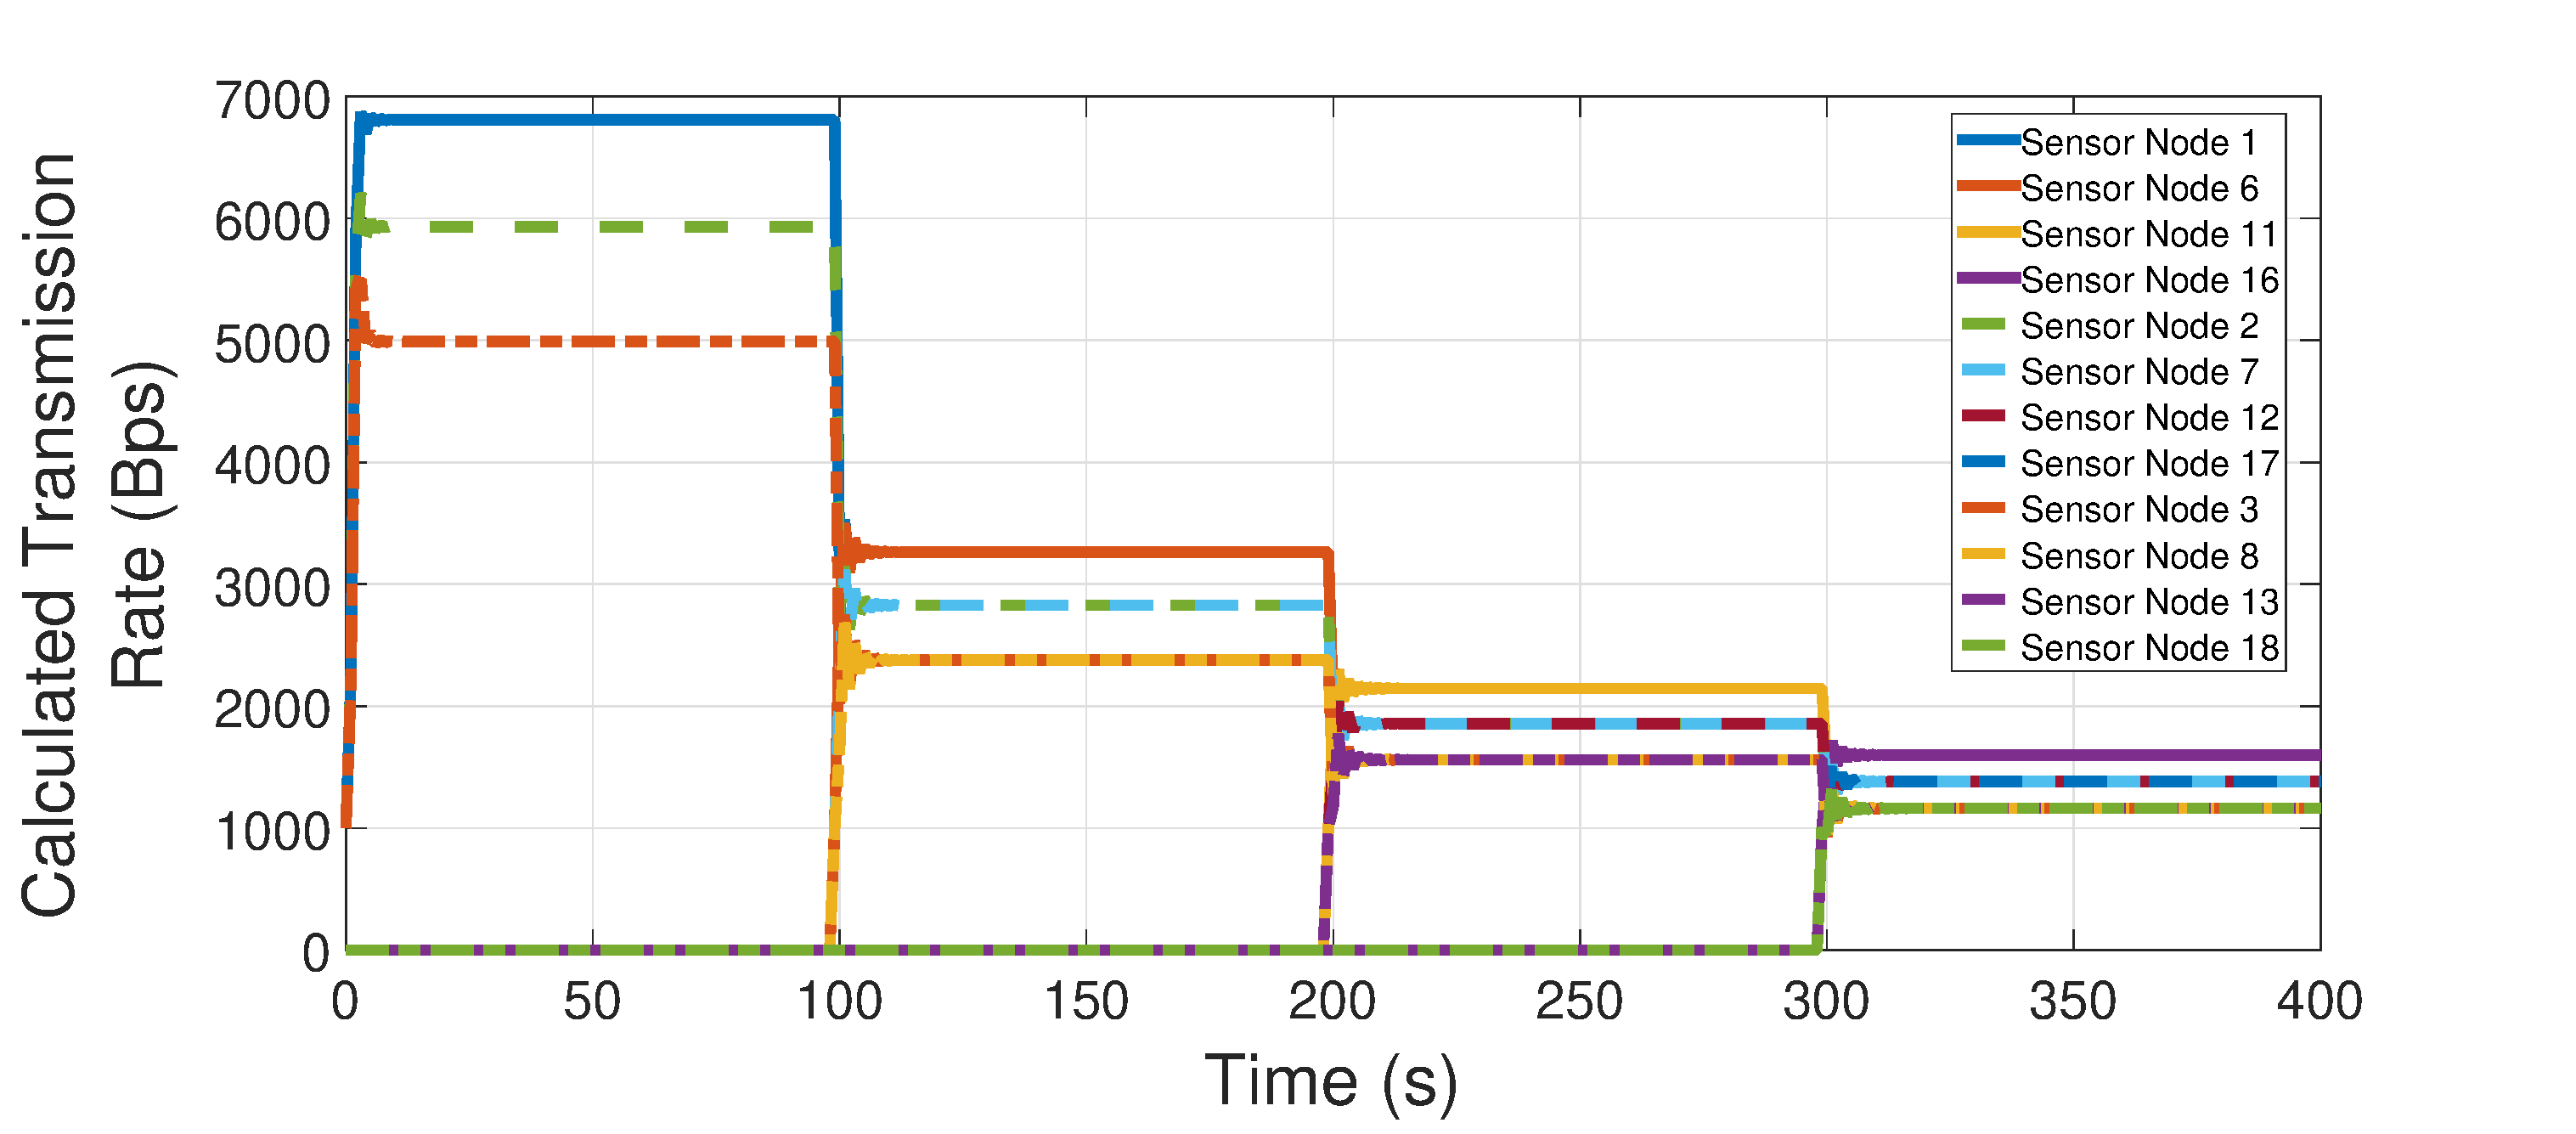
\includegraphics[width=1\linewidth]{pics/comp2}
	\caption{Comparing there different priority class}
	\label{fig:comp2}
\end{figure}